\documentclass[11pt, twoside]{memoir}

\setsecnumdepth{subsubsection}
\settocdepth{subsubsection}

\usepackage[normalem]{ulem}

\usepackage{fontspec}
	\setmainfont%
		[Mapping=tex-text]
	{Cambria}
	\setsansfont%
%	[Ligatures={NoCommon, NoDiscretionary},%
		[Mapping=tex-text]%
		{Inconsolata}
\usepackage{relsize}

\def\textlabel#1{{\relsize{-.5}\fontspec[Mapping=tex-text]{Roboto Mono}{#1}}}
\def\langtext#1{\textit{#1}}

\usepackage{float}

\usepackage[top=1in, bottom=1in, left=1.25in, right=1.25in]{geometry}

\usepackage{xcolor}

\usepackage{hyperref}

\renewcommand\cftappendixname{\appendixname~}
\usepackage[nonumberlist, nopostdot, section=chapter, numberedsection=autolabel]{glossaries}
\makeglossaries

\usepackage{tikz}
\usetikzlibrary{shapes, arrows, backgrounds, fit, positioning}
\usetikzlibrary{decorations.pathreplacing}
\tikzset{
    dots/.style={
        line width=4pt,
        line cap=round,
        dash pattern=on 0pt off 6pt
    }
}
\usepackage{colortbl}
	\definecolor{CB1}{RGB}{0, 114, 178}%BLUE
	\definecolor{CB2}{RGB}{213, 94, 0}%VERMILLION
	\definecolor{CB3}{RGB}{0, 158, 115}%BLUE GREEN
	\definecolor{CB4}{RGB}{204, 121, 167}%REDDISH PURPLE
	\definecolor{CB5}{RGB}{86, 180, 233}%SKY BLUE
	\definecolor{CB6}{RGB}{230, 159, 0}%ORANGE
	\definecolor{CB7}{RGB}{240, 228, 66}%YELLOW
	\def\CB#1#2{\textcolor{CB#1}{#2}}
\usepackage{booktabs, longtable, array, arydshln, multirow}
\usepackage{caption}
\newlength\defaultaboverulesep
\setlength\defaultaboverulesep{\aboverulesep}
\newlength\defaultbelowrulesep
\setlength\defaultbelowrulesep{\belowrulesep}
\setlength\aboverulesep{0pt}
\setlength\belowrulesep{0pt}
\def\arraystretch{1.15}

\usepackage[framemethod=tikz]{mdframed}
	\newmdenv[middlelinecolor=CB1,
		middlelinewidth=1pt,
		backgroundcolor=gray!50,
		roundcorner=4pt]{infobox}
	\newmdenv[middlelinecolor=CB2,
		middlelinewidth=2pt,
		backgroundcolor=CB2!30,
		roundcorner=4pt]{toexpand}

\usepackage{makeidx}
\usepackage{graphicx}
	\graphicspath{{figures}}

\usepackage{expex}

\usepackage{enumitem}
	\setitemize{itemsep=.5ex, topsep=1ex, parsep=0pt, partopsep=0pt, leftmargin=3em, rightmargin=0ex}
	\setenumerate{itemsep=.5ex, topsep=1ex, parsep=0pt, partopsep=0pt, leftmargin=3em, rightmargin=0em}
\usepackage[hang, flushmargin, multiple, bottom, stable]{footmisc}

\usepackage{fancyhdr}

\usepackage{natbib}
	\bibpunct[:]{(}{)}{,}{a}{}{,}
	\setlength{\bibsep}{1ex plus 0.3ex}
\renewcommand{\bibsection}{\part*{Bibliography}}

\usepackage{cite-ref-errors}

\setlength\parskip{.5\baselineskip}
\setlength\parindent{0pt}
\frenchspacing
\raggedbottom

\def\THIStitle{Embarking on PoLaR Explorations}
\def\THISsubtitle{A Framework for Intonational Annotation and Analysis}
\pagestyle{fancy}
	\fancyhead[LO]{\textit{\THIStitle}}
	\fancyhead[RO]{}
	\fancyhead[LE]{}
	\fancyhead[RE]{Ahn, Veilleux, Shattuck-Hufnagel, Brugos}
\pagestyle{plain}
\hypersetup{
	breaklinks=true,
	pdfauthor={Byron Ahn, Nanette Veilleux, Stefanie Shattuck-Hufnagel, and Alejna Brugos},
	pdftitle={\THIStitle: \THISsubtitle},
	bookmarks,
	bookmarksopen=true,
	colorlinks=false,
	allcolors=blue
}

\makeindex

\begin{document}
\frontmatter
\captionsetup{margin=1.5cm, skip=4pt, labelfont={bf, footnotesize}, textfont={footnotesize}}

\title{\THIStitle}
\author{Byron Ahn \and Nanette Veilleux \and Stefanie Shattuck-Hufnagel \and Alejna Brugos}
\date{\today}
%{\normalsize\textcolor{red}{These guidelines are still under active development.\\Find the latest version of the guidelines, as well as .wav files, .TextGrid files, and some scripts, at \url{https://www.polarlabels.com/}.}}

\begin{titlingpage}
\vspace*{\fill}
\begin{center}
\textbf{\huge{\THIStitle:\strut}}\\
\textbf{\huge{\THISsubtitle\strut}}
\\[6\baselineskip]
{\large{Byron Ahn,\strut\\Nanette Veilleux,\strut\\Stefanie Shattuck-Hufnagel,\strut\\and Alejna Brugos\strut}}\\[6\baselineskip]
{\large\textit{draft}}\\
November 2022
\end{center}
\vspace*{\fill}
\end{titlingpage}

\tableofcontents
\newpage
\listoffigures
\listoftables
\newpage

\mainmatter
\chapter{Usage Cases for PoLaR}\label{ch:advantages}

Having reviewed the PoLaR annotation framework, we turn now to some contexts where we see PoLaR as being particularly useful.

A practitioner of prosodic labelling often has a persistent sense that (i) there are systematic differences (possibly implementational, possibly contrastive) that are not being captured; (ii) difficult-to-label tokens may be pointing to ways in which the theoretical framework can be revised or extended; and (iii) aspects of inter-labeller disagreement could be (and ought to be) lessened. Moreover, the practitioner may have the sense that, generally, these concerns could be addressed if there were a) appropriate phonetic labels that more transparently reflect observable aspects of the signal, and b) more widespread consideration of the possibility that different speakers, listeners (and labellers) may use the different cues to prosodic constituent structure and prominence in different ways.

A wide variety of research contexts are to some extent entangled in all of these issues; in this section we briefly discuss some of the ways in which PoLaR can help to address them, largely because it provides more information about the phonetic realization of a prosodic contour. These advantages include capturing systematic variation (e.g. in pitch slopes, pitch contours, pitch ranges, and cross-speaker differences in implementing a phonological category), and a minimization of labelling-related issues (e.g., labeller uncertainty or inter-labeller disagreement). We also discuss the ways in which this annotation framework makes the development of labelling skills more accessible to new labellers, and how it can be used in contexts where categorical labels are not suitable (such as exploration of an understudied variety or language). 


\section{Capturing systematic variation}\label{sec:capturing-systematic-variation}

\subsection{Exploring the Intonational Phonetics-Phonology Interface}\label{sec:exploring-phonetics-phonology-interface}
PoLaR labelling can be thought of as capturing a set of acoustic\slash perceptual characteristics of intonation in a way that is different from phonological labelling systems (like MAE\_ToBI) that aim to capture discrete phonological units. A researcher using the latter sort of labelling may benefit from the additional information captured by PoLaR labels in two ways. First, PoLaR labels capture more details about the relevant raw acoustic cues (e.g., going beyond “High” and “Low” to include scaled pitch level and the size of the pitch range it occurs in), which can be useful to help understand how phonemic categories are phonetically realized. Second, PoLaR can be used to systematically explore the predictions and/or adequacy of a particular categorical labelling system, with respect to its adopted phonemic inventory or phonological model.

As a concrete example for this general description, consider two cases where the conventions of MAE\_ToBI labelling (by design) collapse a range of acoustic realizations. In each of Fig. \ref{fig:final low Usages} and Fig. \ref{fig:sagging Usages} below, multiple possible f0 tracks are depicted, and the same set of MAE\_ToBI labels (/\textlabel{H* H* L-L\%}/) would be used to capture them.

\begin{figure}[H]
\centering
%
\tikzset{
    dots/.style={
        line width=4pt,
        line cap=round,
        dash pattern=on 0pt off 6pt
    }
}
\begin{tikzpicture}[scale=1.25]
%\node[anchor=north west, xscale=.225, yscale=.225] at (-0.525,4.15) {\includegraphics{ranges-what-if4.png}};
\node[rotate=90] at (-0.75,3) {\relsize{-2}f0 (Hz)};
\begin{scope}[anchor=east, style={font=\relsize{-2}}]
%	\node at (0,0) {0};
%	\node at (0,1) {100};
	\node at (0,2) {200};
	\node at (0,3) {300};
	\node at (0,4) {400};
\end{scope}
\foreach \y in {2,...,4}
{
	\draw (0,\y) -- (-.1,\y);
}
\begin{scope}
\draw (0,4.25) rectangle (6.4,1.75);
\draw (0.0,1.75) rectangle (1.6,1.25);
\node at (.8, 1.5) {\relsize{-2}word1};
\draw (1.6,1.75) rectangle (3.2,1.25);
\node at (2.4, 1.5) {\relsize{-2}word2};
\draw (3.2,1.75) rectangle (4.8,1.25);
\node at (4, 1.5) {\relsize{-2}word3};
\draw (4.8,1.75) rectangle (6.4,1.25);
\node at (5.6, 1.5) {\relsize{-2}word4};
%
\draw (0,1.25) rectangle (6.4,0.75);
\draw (1.3, 1.25) -- (1.3, 0.75);
\node[fill=white] at (1.3, 1) {\relsize{-2}H*};
\draw (2.8, 1.25) -- (2.8, 0.75);
\node[fill=white] at (2.8, 1) {\relsize{-2}H*};
\draw (6.05, 1.25) -- (6.05, 0.75);
\node[fill=white] at (6.05, 1) {\relsize{-2}L-L\%};
%
\coordinate (pt1) at (0.2,2.85);
\coordinate (pt2) at (1.4,3.95);
\coordinate (pt3) at (2.8,3.95);
\coordinate (pt4) at (3.95,2.25);
\coordinate (pt5) at (6.2,2.25);
\coordinate (pt5a) at (5.2,2.25);
\coordinate (pt5b) at (6.1,1.85);
%\foreach \x in {1,...,14}
%{
%	\draw[fill] (pt\x) circle (.05);
%}
\draw[CB1, dots] (pt1) sin (pt2) -- (pt3) cos ([xshift=0,yshift=7]pt4) sin ([xshift=7,yshift=0]pt4) -- (pt5);
\draw[CB2, line width=2.33pt, line cap=round, dashed] (pt1) sin (pt2) -- (pt3) cos ([xshift=0,yshift=7]pt4) sin ([xshift=7,yshift=0]pt4) -- (pt5a) -- (pt5b);
\end{scope}
\end{tikzpicture}
%
\caption{The final low plateau and low plateau with an extra fall have conventionally been labelled as \textlabel{L-L\%} in MAE\_ToBI.%
\label{fig:final low Usages}%
%\index{Annotated example, Usage cases!XXX}
}
\end{figure}

\begin{figure}[H]
\centering
%
\tikzset{
    dots/.style={
        line width=4pt,
        line cap=round,
        dash pattern=on 0pt off 6pt
    }
}
\begin{tikzpicture}[scale=1.25]
%\node[anchor=north west, xscale=.225, yscale=.225] at (-0.525,4.15) {\includegraphics{ranges-what-if4.png}};
\node[rotate=90] at (-0.75,3) {\relsize{-2}f0 (Hz)};
\begin{scope}[anchor=east, style={font=\relsize{-2}}]
%	\node at (0,0) {0};
%	\node at (0,1) {100};
	\node at (0,2) {200};
	\node at (0,3) {300};
	\node at (0,4) {400};
\end{scope}
\foreach \y in {2,...,4}
{
	\draw (0,\y) -- (-.1,\y);
}
\begin{scope}
\draw (0,4.25) rectangle (6.4,1.75);
\draw (0.0,1.75) rectangle (1.6,1.25);
\node at (.8, 1.5) {\relsize{-2}word1};
\draw (1.6,1.75) rectangle (3.2,1.25);
\node at (2.4, 1.5) {\relsize{-2}word2};
\draw (3.2,1.75) rectangle (4.8,1.25);
\node at (4, 1.5) {\relsize{-2}word3};
\draw (4.8,1.75) rectangle (6.4,1.25);
\node at (5.6, 1.5) {\relsize{-2}word4};
%
\draw (0,1.25) rectangle (6.4,0.75);
\draw (1.3, 1.25) -- (1.3, 0.75);
\node[fill=white] at (1.3, 1) {\relsize{-2}H*};
\draw (2.8, 1.25) -- (2.8, 0.75);
\node[fill=white] at (2.8, 1) {\relsize{-2}H*};
\draw (6.05, 1.25) -- (6.05, 0.75);
\node[fill=white] at (6.05, 1) {\relsize{-2}L-L\%};
%
\coordinate (pt1) at (0.2,2.85);
\coordinate (pt2) at (1.4,3.95);
\coordinate (pt2a) at (2.1,3.45);
\coordinate (pt2b) at (2.1,3);
\coordinate (pt3) at (2.8,3.95);
\coordinate (pt4) at (3.95,2.25);
\coordinate (pt5) at (6.2,2.25);
%\foreach \x in {1,...,14}
%{
%	\draw[fill] (pt\x) circle (.05);
%}
\draw[CB1, dots] (pt1) sin (pt2) -- (pt3) cos ([xshift=0,yshift=7]pt4) sin ([xshift=7,yshift=0]pt4) -- (pt5);
\draw[CB3, line width=2.33pt, line cap=round, dashed] (pt1) sin (pt2) cos ([xshift=-5,yshift=2]pt2a) sin (pt2a) cos ([xshift=5,yshift=2]pt2a) sin (pt3) cos ([xshift=0,yshift=7]pt4) sin ([xshift=7,yshift=0]pt4) -- (pt5);
\draw[CB4, line width=2pt, dotted] (pt1) sin (pt2) cos ([xshift=-5,yshift=2]pt2b) sin (pt2b) cos ([xshift=5,yshift=2]pt2b) sin (pt3) cos ([xshift=0,yshift=7]pt4) sin ([xshift=7,yshift=0]pt4) -- (pt5);
\end{scope}
\end{tikzpicture}
%
\caption{A contour with two High pitch accents (MAE\_ToBI: \textlabel{H*}) can variably have a plateau between corresponding peaks or various degrees of sagging between them.%
\label{fig:sagging Usages}%
%\index{Annotated example, Usage cases!XXX}
}
\end{figure}

Using PoLaR’s (mostly phonetic) labels alongside phonemic labels like ToBI’s could help explore systematicity in the phonetic variation within theses phonemic labels. For example, in the case of Fig. \ref{fig:final low Usages}, PoLaR Points, Levels, and Ranges labels would be differ between the two contours, potentially uncovering systematicity in how \textlabel{L-L\%} is realized. In the case of Fig. \ref{fig:sagging Usages}, such sagging has been argued to be surface variation of the same phonological sequence of \textlabel{H*}s; PoLaR Points and Levels Ranges labels may help to uncover whether there is systematicity about the degree, timing, and depth of such sags.

In addition, such work (or even work where PoLaR labels alone are annotated) may even possibly uncover new phonemic distinctions. For example, there may be phenomena that have been treated as category-internal variation (e.g., \textlabel{L-L\%} realized as either a final fall or low plateau, or various degrees of sags between \textlabel{H*}s) where the variation turns out to be contextually-determined; and if the relevant contextual variables are semantic\slash pragmatic, this could be analyzed as an undiagnosed phonemic distinction, which in turn could be used to argue for readjusting the intonational phonemic inventory of the language.

More broadly, using PoLaR (alongside independently annotated categorical labels) facilitates exploring questions about what sort of variation there is within-category, in the domain of intonation. In addition to the sorts of questions asked for the figures above, side-by-side usage of PoLaR and phonemic labels could explore questions like:

\begin{itemize}
	\item At what rate do accents like \textlabel{L*} or \textlabel{H*} get realized with each of the possible Levels values?
	\item How do peaks\slash valleys (as labelled on the Points tier) align with Phone segments that are marked with a pitch accent label like \textlabel{H*} or \textlabel{L*}?
	\item How are the beginnings of phrase-final boundary plateaus (ToBI \textlabel{H-} and \textlabel{L-}) timed with respect to Phones segments and/or PrStr \textlabel{*} and \textlabel{]} labels?
	\item etc.
\end{itemize}

In other words, PoLaR enables users to systematically annotate a variety of cues (including those that a labeller attends to when choosing each phonological label) in a way that can be used to track potentially systematic variation (even in post-hoc analysis). To sum up why this type of more detailed labelling is important: it is impossible to discover which differences are systematic if the differences are not tracked (e.g., with annotation).


\subsection{Slopes in f0 movements}\label{sec:pitch-slopes}
As discussed above, many types of variation are potentially systematic and context-governed but are not possible to capture with a phonological labelling system, which by definition asks its users to lump together a variety of realizations under each of a particular set of predefined categorical labels. A categorical labelling system would not, by design, distinguish all degrees of phrase-final rises or of phrase-final falls. However, it may still be an open question how many communicatively different degrees of rise or of fall exist. For example, does the difference between boundary-related low flat f0 and a low but falling final f0 (as depicted in Figure \ref{fig:final low Usages}, above) convey a difference in meaning, or are these likely to be used in different contexts? If so, the categorical labels ought to reflect such a difference. However, answering questions like this, about the phonetics-phonology interface, requires keeping track of degrees of final rises\slash falls systematically.

The PoLaR Levels tier (and indirectly the Points and Ranges tiers) can facilitate just this. For example, these labels distinguish a rise from level 3 to level 5 and a rise from level 1 to level 5, or a low flat final f0 from one with an additional final fall on the last syllable. PoLaR makes these scaled levels of pitch explicit, which facilitates exploration of how many categories of rise or fall need to be described by the phonology, by making it possible to look at how the acoustically-different realizations cluster. Doing this kind of tracking may be familiar to many researchers, who measure phrase-final f0 movements as occurring over intervals of some particular operationally-defined size. Though this can of course be done without PoLaR, PoLaR can streamline this process. Namely, since Points\slash Levels tier labels already track where f0 changes slope, they are ideal candidates for defining the endpoints of the interval for phrase-final f0 movements. In summary, using PoLaR labels to define endpoints for f0 slope can add a layer of methodological consistency to defining the interval for such f0 movements.

In addition, given that Levels labels are “scaled” (i.e., normalized, based on the Ranges tier labels), the rate of change calculated from Levels may facilitate comparison across individuals and/or recordings. Imagine the two hypothetical utterances shown below:

\begin{figure}[H]
\centering
%
\begin{tikzpicture}[scale=.85, transform shape]%\node[anchor=north west, xscale=.225, yscale=.225] at (-0.525,4.15) {\includegraphics{ranges-what-if5.png}};
\node[rotate=90] at (-0.75,3) {\relsize{-2}f0 (Hz)};
\begin{scope}[anchor=east, style={font=\relsize{-2}}]
%	\node at (0,0) {0};
	\node at (0,1) {100};
	\node at (0,2) {200};
	\node at (0,3) {300};
	\node at (0,4) {400};
\end{scope}
\foreach \y in {1,...,4}
{
	\draw (0,\y) -- (-.1,\y);
}
\begin{scope}
\draw (0,4.25) rectangle (7.75,.5);
\draw (0,0) rectangle (7.75,.5);
\node at (3.875, .25) {\relsize{-2}100-400};
\coordinate (pt0) at (0.2,1.5);
\coordinate (pt1) at (1.2,1.85);
\coordinate (pt2) at (1.7,3.0);
\coordinate (pt3) at (2.4,1.45);
\coordinate (pt4) at (3,1.15);
\coordinate (pt5) at (6,1.05);
\coordinate (pt6) at (7,3.95);
%\coordinate (pt7) at (5.3,2.25);
%\coordinate (pt8) at (6.4,2.25);
%\coordinate (pt9) at (7.45,2.2);
%\foreach \x in {1,...,9}
%{
%	\draw[fill] (pt\x) circle (.05);
%}
\draw[CB1, dots] (pt0) cos (pt1) sin (pt2) cos (pt3) sin  (pt4) cos (pt5) cos (pt6);
%\draw[CB1, dots] (pt7) .. controls (pt8) .. (pt9);
\end{scope}
\begin{scope}[style={font=\relsize{-1}}]
\draw[red, fill = red, fill opacity = .35] (6,.95) rectangle (7.1,4.05);
\node [red, anchor=north] at (6.5, .95) {250ms};
\node [red, rotate = 90, anchor=north] at (7.1, 2.5) {300Hz};
\end{scope}
%\begin{scope}[very thick, red]
%\draw [decorate, decoration = {brace, mirror}] (6,.85) --  (7,.85);	
%\end{scope}\end{tikzpicture}~~\begin{tikzpicture}[scale=.85, transform shape]%\node[anchor=north west, xscale=.225, yscale=.225] at (-0.525,4.15) {\includegraphics{ranges-what-if5.png}};
\node[rotate=90] at (-0.75,3) {\relsize{-2}f0 (Hz)};
\begin{scope}[anchor=east, style={font=\relsize{-2}}]
%	\node at (0,0) {0};
	\node at (0,1) {100};
	\node at (0,2.5) {150};
%	\node at (0,3) {300};
	\node at (0,4) {200};
\end{scope}
%\foreach \y in {1,...,3}
%{
	\draw (0,1) -- (-.1,1);
	\draw (0,2.5) -- (-.1,2.5);
	\draw (0,4) -- (-.1,4);
%}
\begin{scope}
\draw (0,4.25) rectangle (7.75,.5);
\draw (0,0) rectangle (7.75,.5);
\node at (3.875, .25) {\relsize{-2}100-200};
\coordinate (pt0) at (0.2,1.5);
\coordinate (pt1) at (1.2,1.85);
\coordinate (pt2) at (1.7,3.0);
\coordinate (pt3) at (2.4,1.45);
\coordinate (pt4) at (3,1.15);
\coordinate (pt5) at (6,1.05);
\coordinate (pt6) at (7,3.95);
%\coordinate (pt7) at (5.3,2.25);
%\coordinate (pt8) at (6.4,2.25);
%\coordinate (pt9) at (7.45,2.2);
%\foreach \x in {1,...,9}
%{
%	\draw[fill] (pt\x) circle (.05);
%}
\draw[CB1, dots] (pt0) cos (pt1) sin (pt2) cos (pt3) sin  (pt4) cos (pt5) cos (pt6);
%\draw[CB1, dots] (pt7) .. controls (pt8) .. (pt9);
\end{scope}
\begin{scope}[style={font=\relsize{-1}}]
\draw[red, fill = red, fill opacity = .35] (6,.95) rectangle (7.1,4.05);
\node [red, anchor=north] at (6.5, .95) {250ms};
\node [red, rotate = 90, anchor=north] at (7.1, 2.5) {100Hz};
\end{scope}
%\begin{scope}[very thick, red]
%\draw [decorate, decoration = {brace, mirror}] (6,.85) --  (7,.85);	
%\end{scope}\end{tikzpicture}
%
\caption{Two hypothetical utterances that differ primarily in pitch range; note different vertical scales.%
\label{fig:Usages-slopes}%
%\index{Annotated example, Usage cases!XXX}
}
\end{figure}

The difference between the first and second hypothetical utterances is the f0 scaling: as shown by the scale at the left side of each panel and the range markers at the bottom, the former has a pitch range of 100-400Hz, while the latter has a pitch range of 100-200Hz. In terms of PoLaR, these two utterances would be annotated identically, save for Ranges tier. In both cases, the two phrase-final Levels labels would be 1 and 5 (a rise from low to high), Occurring .25sec apart, the slope would be 16 Levels/sec. However, if slope were calculated based on absolute f0 values, the two would have very different slopes: the former would have a slope of 1200Hz/sec, and the latter would have a slope of 400Hz/sec. In other words, because of how Levels labels are calculated relative to the pitch range, Levels labels inherently normalize rate of change in pitch. This is not to say that Levels/sec is a better measure of pitch slope —indeed, Hz/sec (or st/sec) may be more appropriate, at least in some cases— but rather that PoLaR Levels offer a straightforward way to compare pitch contours without additional data wrangling.\footnote{Note that additional time normalization may be desirable for comparisons in some cases, but that is an issue that PoLaR labelling does not directly facilitate.}

Beyond this, if Advanced PoLaR labels are used —in particular Advanced Points labels— then PoLaR provides another advantage: clearly keeping track of which f0 turning points are analyzed as related to prominences and which are related to phrase boundaries. Thus the f0 slopes between intonational events of different types can be tracked. For example, imagine we had the Advanced labels as in Figure \ref{fig:Usages-slopes-advanced}:

\begin{figure}[H]
\centering
%
\begin{tikzpicture}[scale=1.25]%\node[anchor=north west, xscale=.225, yscale=.225] at (-0.525,4.15) {\includegraphics{ranges-what-if5.png}};
\node[rotate=90] at (-0.75,3) {\relsize{-2}f0 (Hz)};
\begin{scope}[anchor=east, style={font=\relsize{-2}}]
%	\node at (0,0) {0};
	\node at (0,1) {100};
	\node at (0,2.5) {150};
%	\node at (0,3) {300};
	\node at (0,4) {200};
\end{scope}
%\foreach \y in {1,...,3}
%{
	\draw (0,1) -- (-.1,1);
	\draw (0,2.5) -- (-.1,2.5);
	\draw (0,4) -- (-.1,4);
%}
\begin{scope}
\draw (0,4.25) rectangle (7.75,.5);

\draw (0,0) rectangle (7.75,.5);
\node[anchor=west] at (7.75,.25) {\relsize{-2}{PrStr}};
\draw (1.5,0) -- node[fill=white]{\relsize{-1}{\texttt{*}}} (1.5,.5);
\draw (7.2,0) -- node[fill=white]{\relsize{-1}{\texttt{]}}} (7.2,.5);

\draw (0,-.5) rectangle (7.75,0);
\node[anchor=west] at (7.75,-.25) {\relsize{-2}{Points}};
\draw (0.2,0) -- node[fill=white]{\relsize{-1}{\texttt{0}}} (0.2,-.5);
\draw (1.1,0) -- node[fill=white]{\relsize{-1}{\texttt{*>}}} (1.1,-.5);
\draw (1.7,0) -- node[fill=white]{\relsize{-1}{\texttt{*<}}} (1.7,-.5);
\draw (2.7,0) -- node[fill=white]{\relsize{-1}{\texttt{]>}}} (2.7,-.5);
%\draw (3,0) -- node[fill=white]{\relsize{-1}{\texttt{0}}} (3,-.5);
\draw (6,0) -- node[fill=white]{\relsize{-1}{\texttt{]>}}} (6,-.5);
\draw (7,0) -- node[fill=white]{\relsize{-1}{\texttt{]>}}} (7,-.5);

\draw (0,-1) rectangle (7.75,-.5);
\node[anchor=west] at (7.75,-.75) {\relsize{-2}{Levels}};
\draw (0.2,-1) -- node[fill=white]{\relsize{-2}{{1}}} (0.2,-.5);
\draw (1.1,-1) -- node[fill=white]{\relsize{-2}{{2}}} (1.1,-.5);
\draw (1.7,-1) -- node[fill=white]{\relsize{-2}{{4}}} (1.7,-.5);
\draw (2.7,-1) -- node[fill=white]{\relsize{-2}{{1}}} (2.7,-.5);
\draw (6,-1) -- node[fill=white]{\relsize{-2}{{1}}} (6,-.5);
\draw (7,-1) -- node[fill=white]{\relsize{-2}{{5}}} (7,-.5);

\draw (0,-1.5) rectangle (7.75,-1);
\node[anchor=west] at (7.75,-1.25) {\relsize{-2}{Ranges}};
\node at (3.875, -1.25) {\relsize{-2}100-200};

\coordinate (pt0) at (0.2,1.5);
\coordinate (pt1) at (1.2,1.85);
\coordinate (pt2) at (1.7,3.0);
\coordinate (pt3) at (2.4,1.45);
\coordinate (pt4) at (3,1.15);
\coordinate (pt5) at (6,1.05);
\coordinate (pt6) at (7,3.95);

\draw[CB1, dots] (pt0) cos (pt1) sin (pt2) cos (pt3) sin  (pt4) cos (pt5) cos (pt6);
\end{scope}\end{tikzpicture}
%
\caption{Advanced PoLaR labels for a hypothetical utterance.%
\label{fig:Usages-slopes-advanced}%
%\index{Annotated example, Usage cases!XXX}
}
\end{figure}

Using these labels, we could measure slopes like the steepness of the rise between the prominence-related Points (the ones labelled here as \textlabel{*>} and \textlabel{*<}), or the steepness of the fall from the last prominence-related Point and the first phrase-related Point (the ones labelled here as \textlabel{*<} and \textlabel{]>}). As before, these are measures that may be familiar to intonationists, but PoLaR labels facilitate finding the relevant endpoints for the measures of slope.

An additional way in which PoLaR can be helpful for calculating f0 slopes is when it comes to files with poor f0 tracking. It is common for those working on f0 measures to need to exclude some number of recordings because of software errors, recording conditions, or microprosodic effects of segments or voice quality. However, because PoLaR labellers can supply comma-override labels in these contexts, many of these files with f0 tracking errors could still be used. For example, the Figure below exhibits f0 tracking errors during “\langtext{out there}”, during which the pitch is perceived to be falling.

\begin{figure}[H]
\centering
%
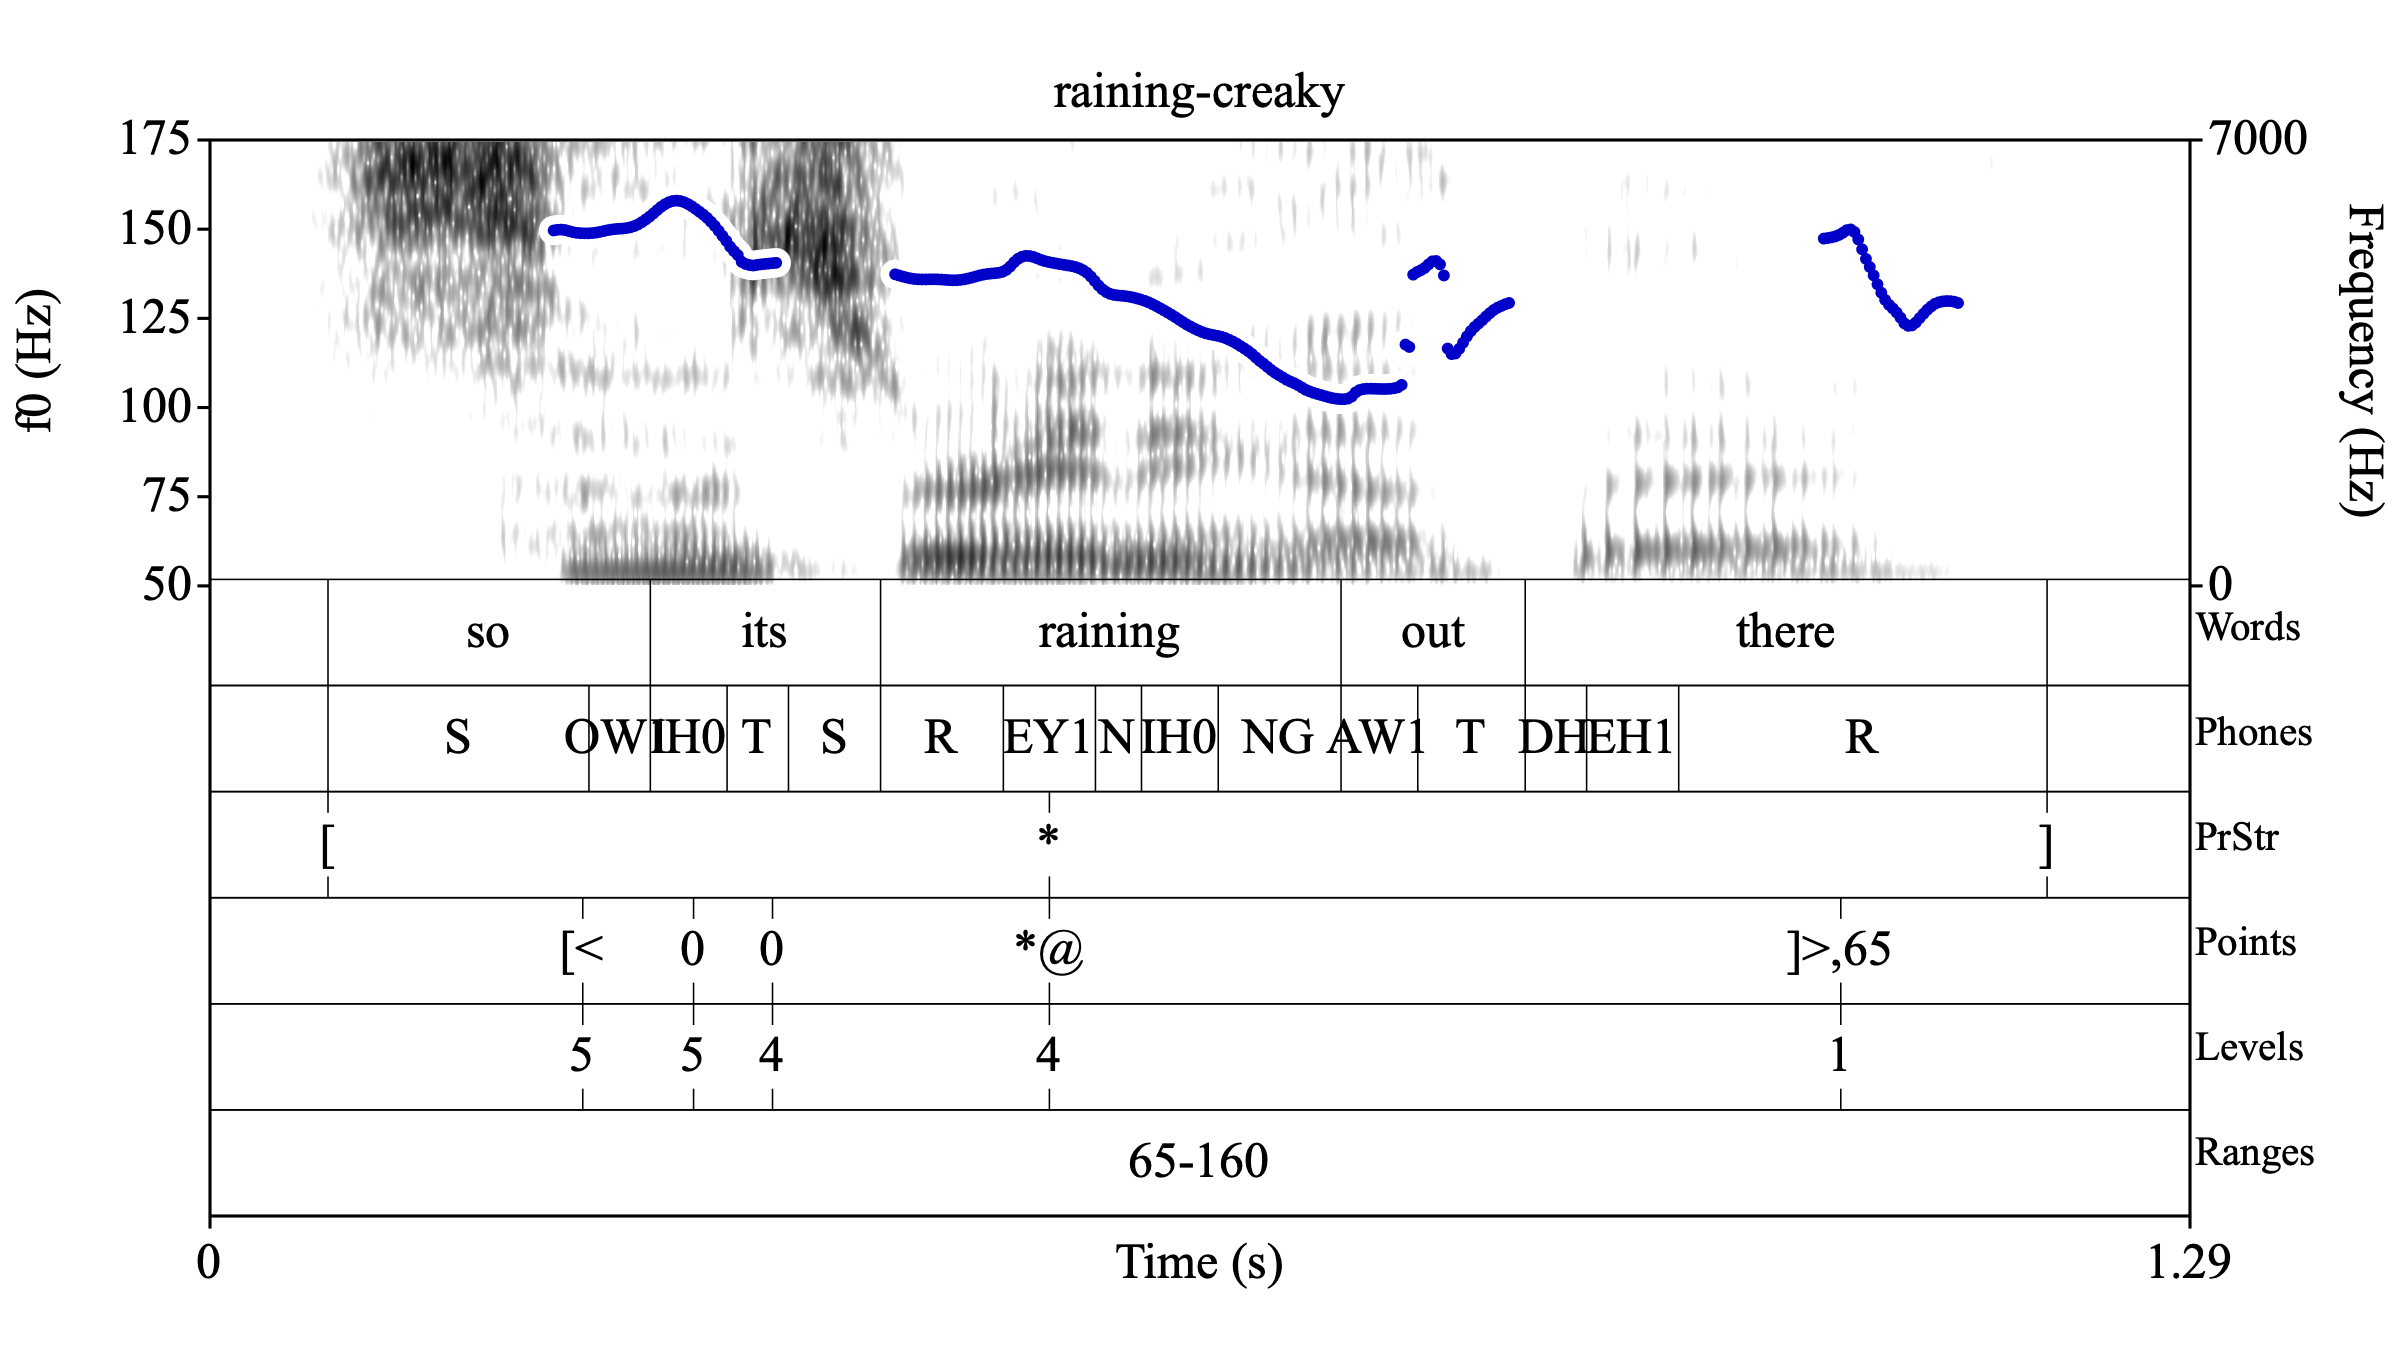
\includegraphics[width=.875\linewidth]{Usages-raining-creaky.png}
%
\caption{The comma override label on the final Points tier object allows the phrase-final movement to be analyzed as falling, potentially avoiding the need to exclude this recording from analysis.%
\label{fig:Usages raining creaky}%
\index{Annotated example, Usage cases!raining-creaky}
}
\end{figure}

Here the f0 at the Points label during “\langtext{raining}” is read as 140.8Hz at 0.547sec, with the final Points label is read as 65Hz (from the comma-override) at 1.290sec – a slope of approximately ​​-102Hz/sec (or in terms of Levels, approximately -4 Levels/sec). Thus comma overrides can be used as a way to include recordings that might otherwise need to be excluded.

\begin{infobox}
For analyses related to slopes of f0 movements, users are encouraged to employ the “Extract info from PoLaR tiers” functionality of the PoLaR plugin for Praat. It can run on an entire directory (or a single file), and for each object on the Points and Levels tiers, it outputs time alignment, f0 value, label, and much more information that can be useful for analysis. It also will respect comma-override labels, and use those values instead of direct measures. Using this and other scripts is briefly discussed in Ch.\ref{ch:practical}, as well as in the plugin documentation.	
\end{infobox}

PoLaR labels can systematically encode listener intuitions relating to the acoustics (such as f0 slope), thus facilitating more targeted acoustic measures. Effectively, PoLaR labels provide more and/or different information than phonological labels do, providing valuable data for the exploration of questions about intonational phonetics and phonology.

\subsection{Intonational Variation across Speakers\slash Varieties\slash Contexts}\label{sec:interspeaker-variation-in-realization-of-prosodic-categories}

Another issue at the phonetics-phonology interface of intonation concerns variation across speakers in the phonetic realization of particular phonological categories. In the fields of phonetics, phonology, and sociolinguistics, a very active area of research explores variation in the realization of particular consonant\slash vowel categories, as well as how the number of phonological categories for consonants and vowels can differ across individuals or varieties. Given that transcription (both narrow and broad) is the first step in doing such comparisons, achieving similar goals in the domain of intonation requires an adequate transcription system. We propose that PoLaR can be useful for the narrower aspects of transcription, while other grammar-oriented transcription systems, like a ToBI system, may be useful for the broader transcription.

As an example, consider the steep-rise pitch accent in American English (in MAE\_ToBI’s broad transcription: /\textlabel{L+H*}/). \citealt{burdin-18} reports on differences in the acoustics of and the frequency of /\textlabel{L+H*}/ in five varieties of English spoken in the U.S. (Jewish English, African American English, Appalachian English, Midland U.S. English, and Southern U.S. English), finding that there are differences in “peak contour height, slope, and peak offset”. Though this work can be done without PoLaR, as discussed in the previous section, PoLaR labelling can be helpful in this domain. Points and Levels tier annotations can be especially useful in calculating f0 height and slope associated with particular phonological events such as pitch accents – especially if Advanced Points labels are used. Points tier annotations can also be used for calculating peak offset, given appropriate Phones tier labels for segment boundaries. (For an example of work that uses PoLaR to explore acoustics of steep-rise pitch accents across contexts and individuals, see \citealt{holliday21a}.)  In addition, if Advanced Points labels are used, one could also track variation in how many turning points are associated with a pitch accent – perhaps some rises involve only two points, but perhaps others (e.g., “scoopy” rises) require more points, or perhaps this varies across varieties. In other words, PoLaR allows researchers to investigate phonetic variation without piecing together annotation methods and ad-hoc practices for phonetic measurement, and without making assumptions that all English varieties share categories, which we return to momentarily.

In addition, Levels labels serve as a transcription of pitch heights beyond raw f0 values that is a narrower transcription than broad categories like H or L. This narrow transcription can be used as a way of clustering different productions together, similar to how narrow-transcription IPA symbols are used to keep track of allophones and their usage in studies on the phonetics-phonology interface or sociolinguistic variation. In this way, one could track the rates at which /\textlabel{L+H*}/ transcriptions are realized as [1-5] rises, [2-4] rises, [3-5] rises, etc, and which contextual variables help to predict how big (in scaled terms) of a rise is used. To be clear, PoLaR can be used alongside phonological systems like ToBI to track which allophones exist and what sociolinguistic variables or contextual conditions from the phonology matter for describing the distribution of the different forms that a phonological object (e.g., a pitch accent) can take.

Below are two recordings of the same line by different speakers, serving as a brief exposition of how PoLaR can be helpful for research questions like this:

\begin{figure}[H]
\centering
%
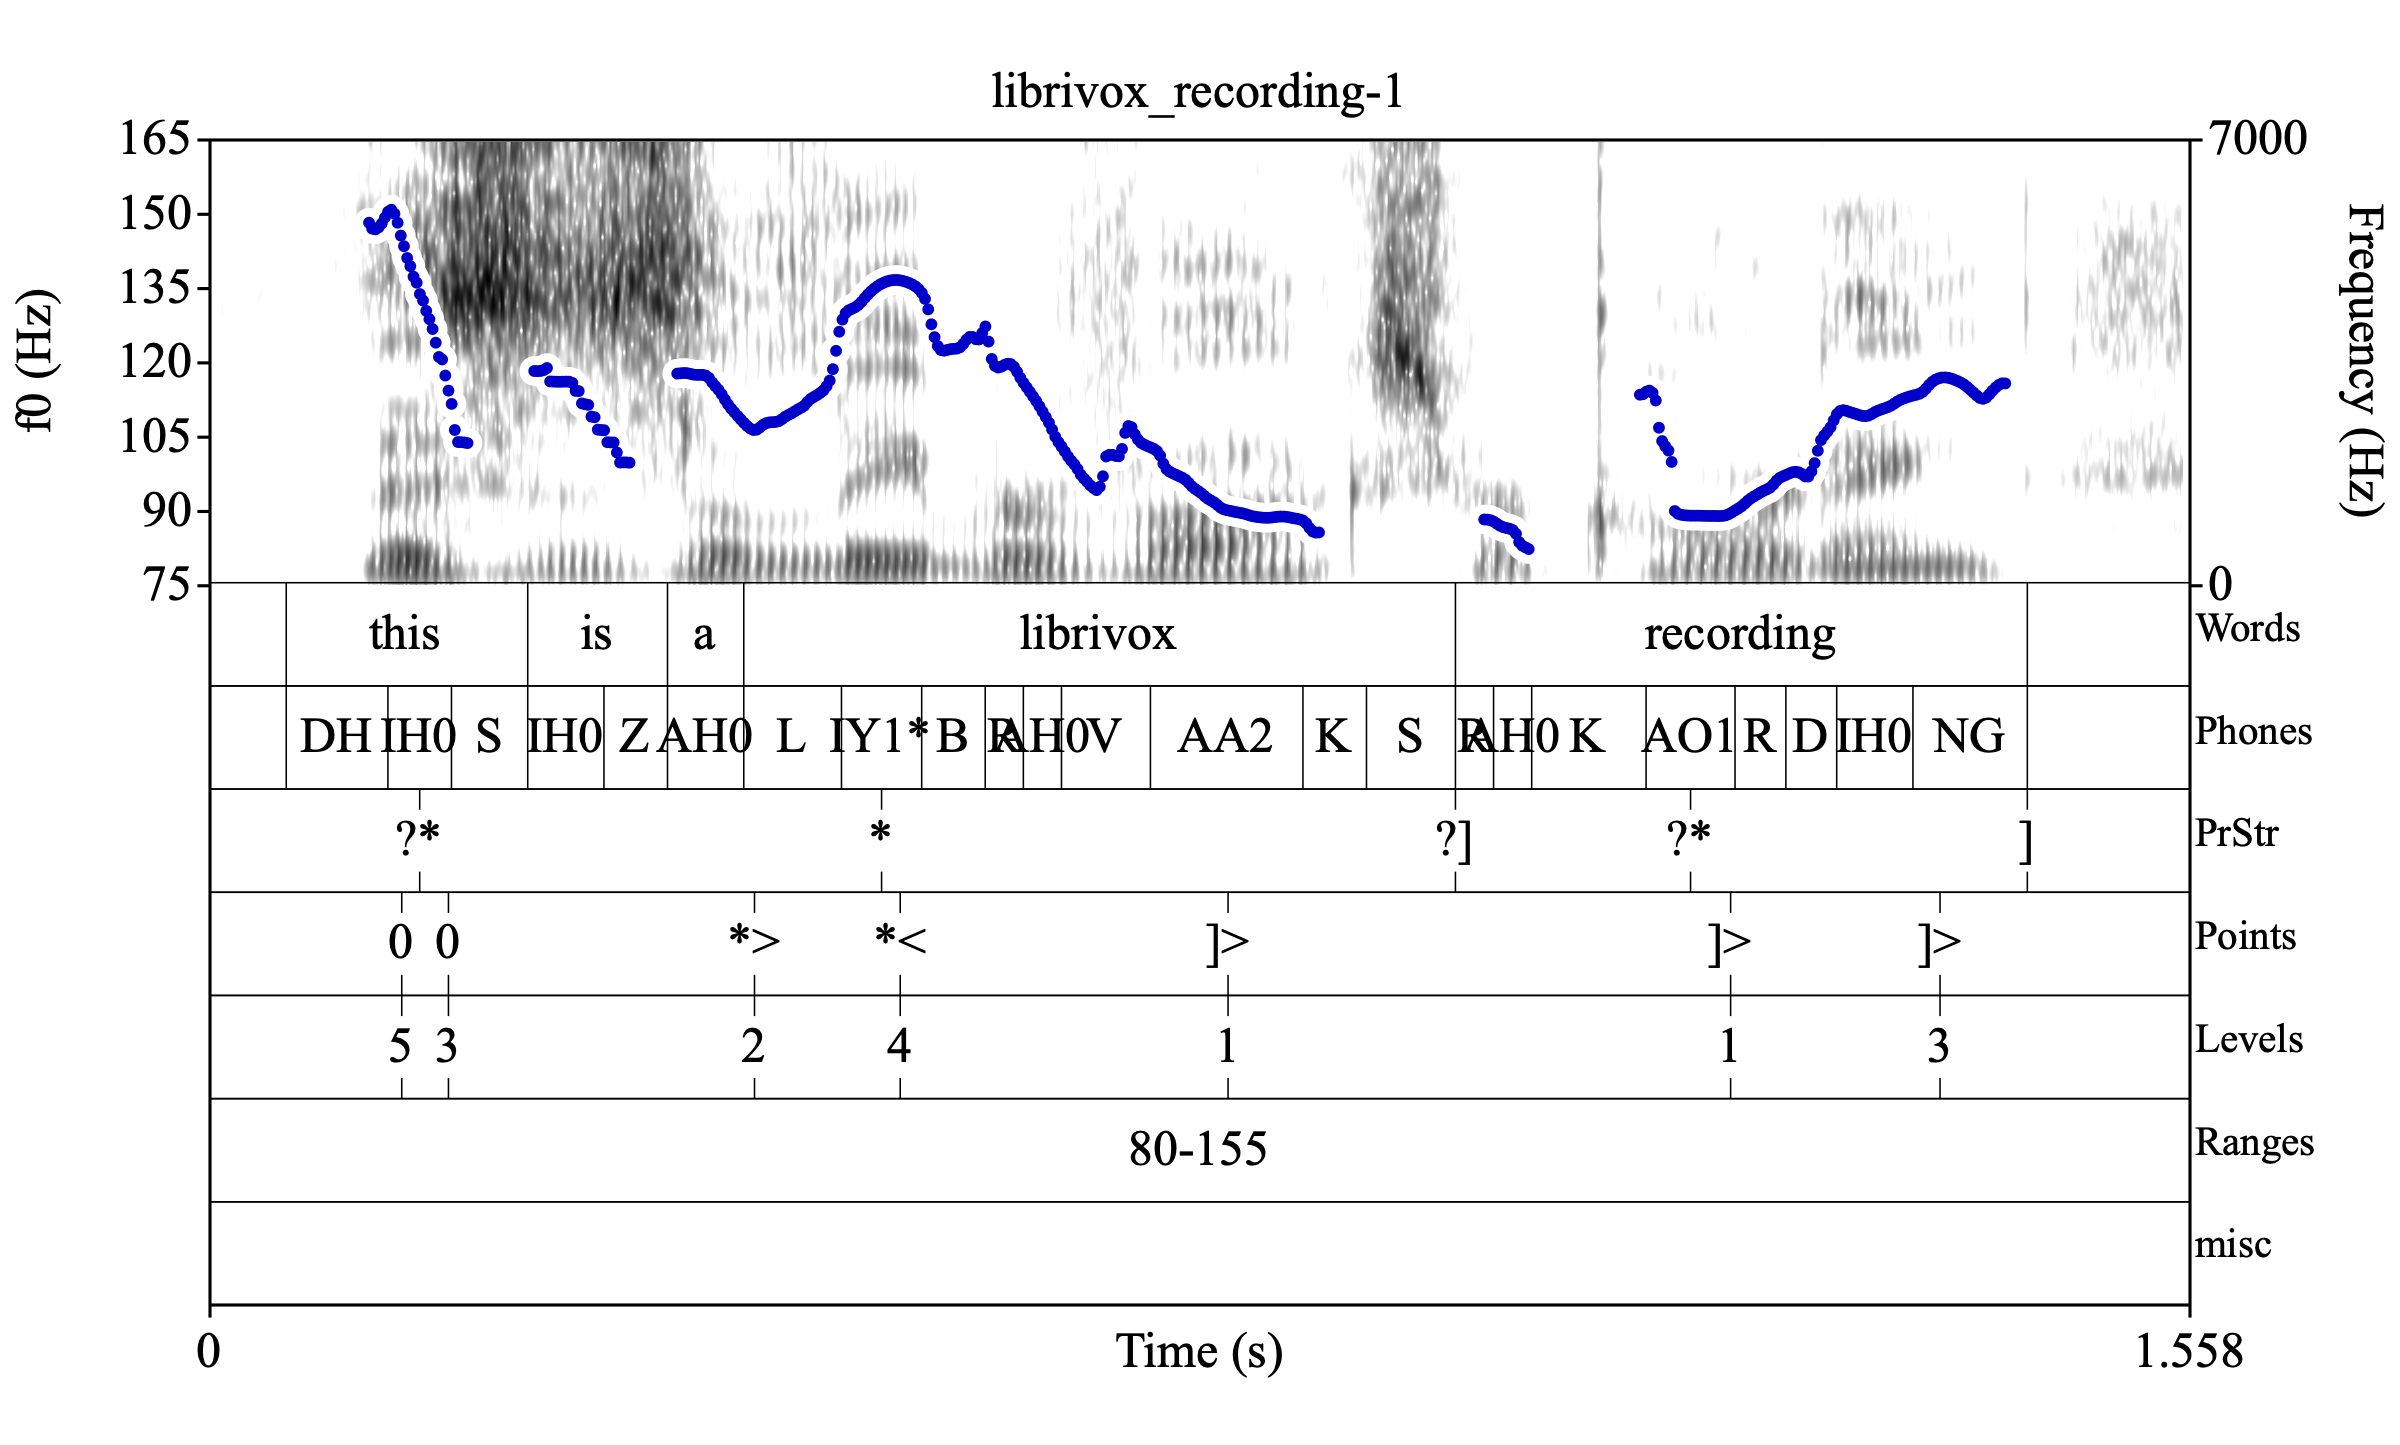
\includegraphics[width=.485\linewidth]{Usages-librivox_recording-1.png} 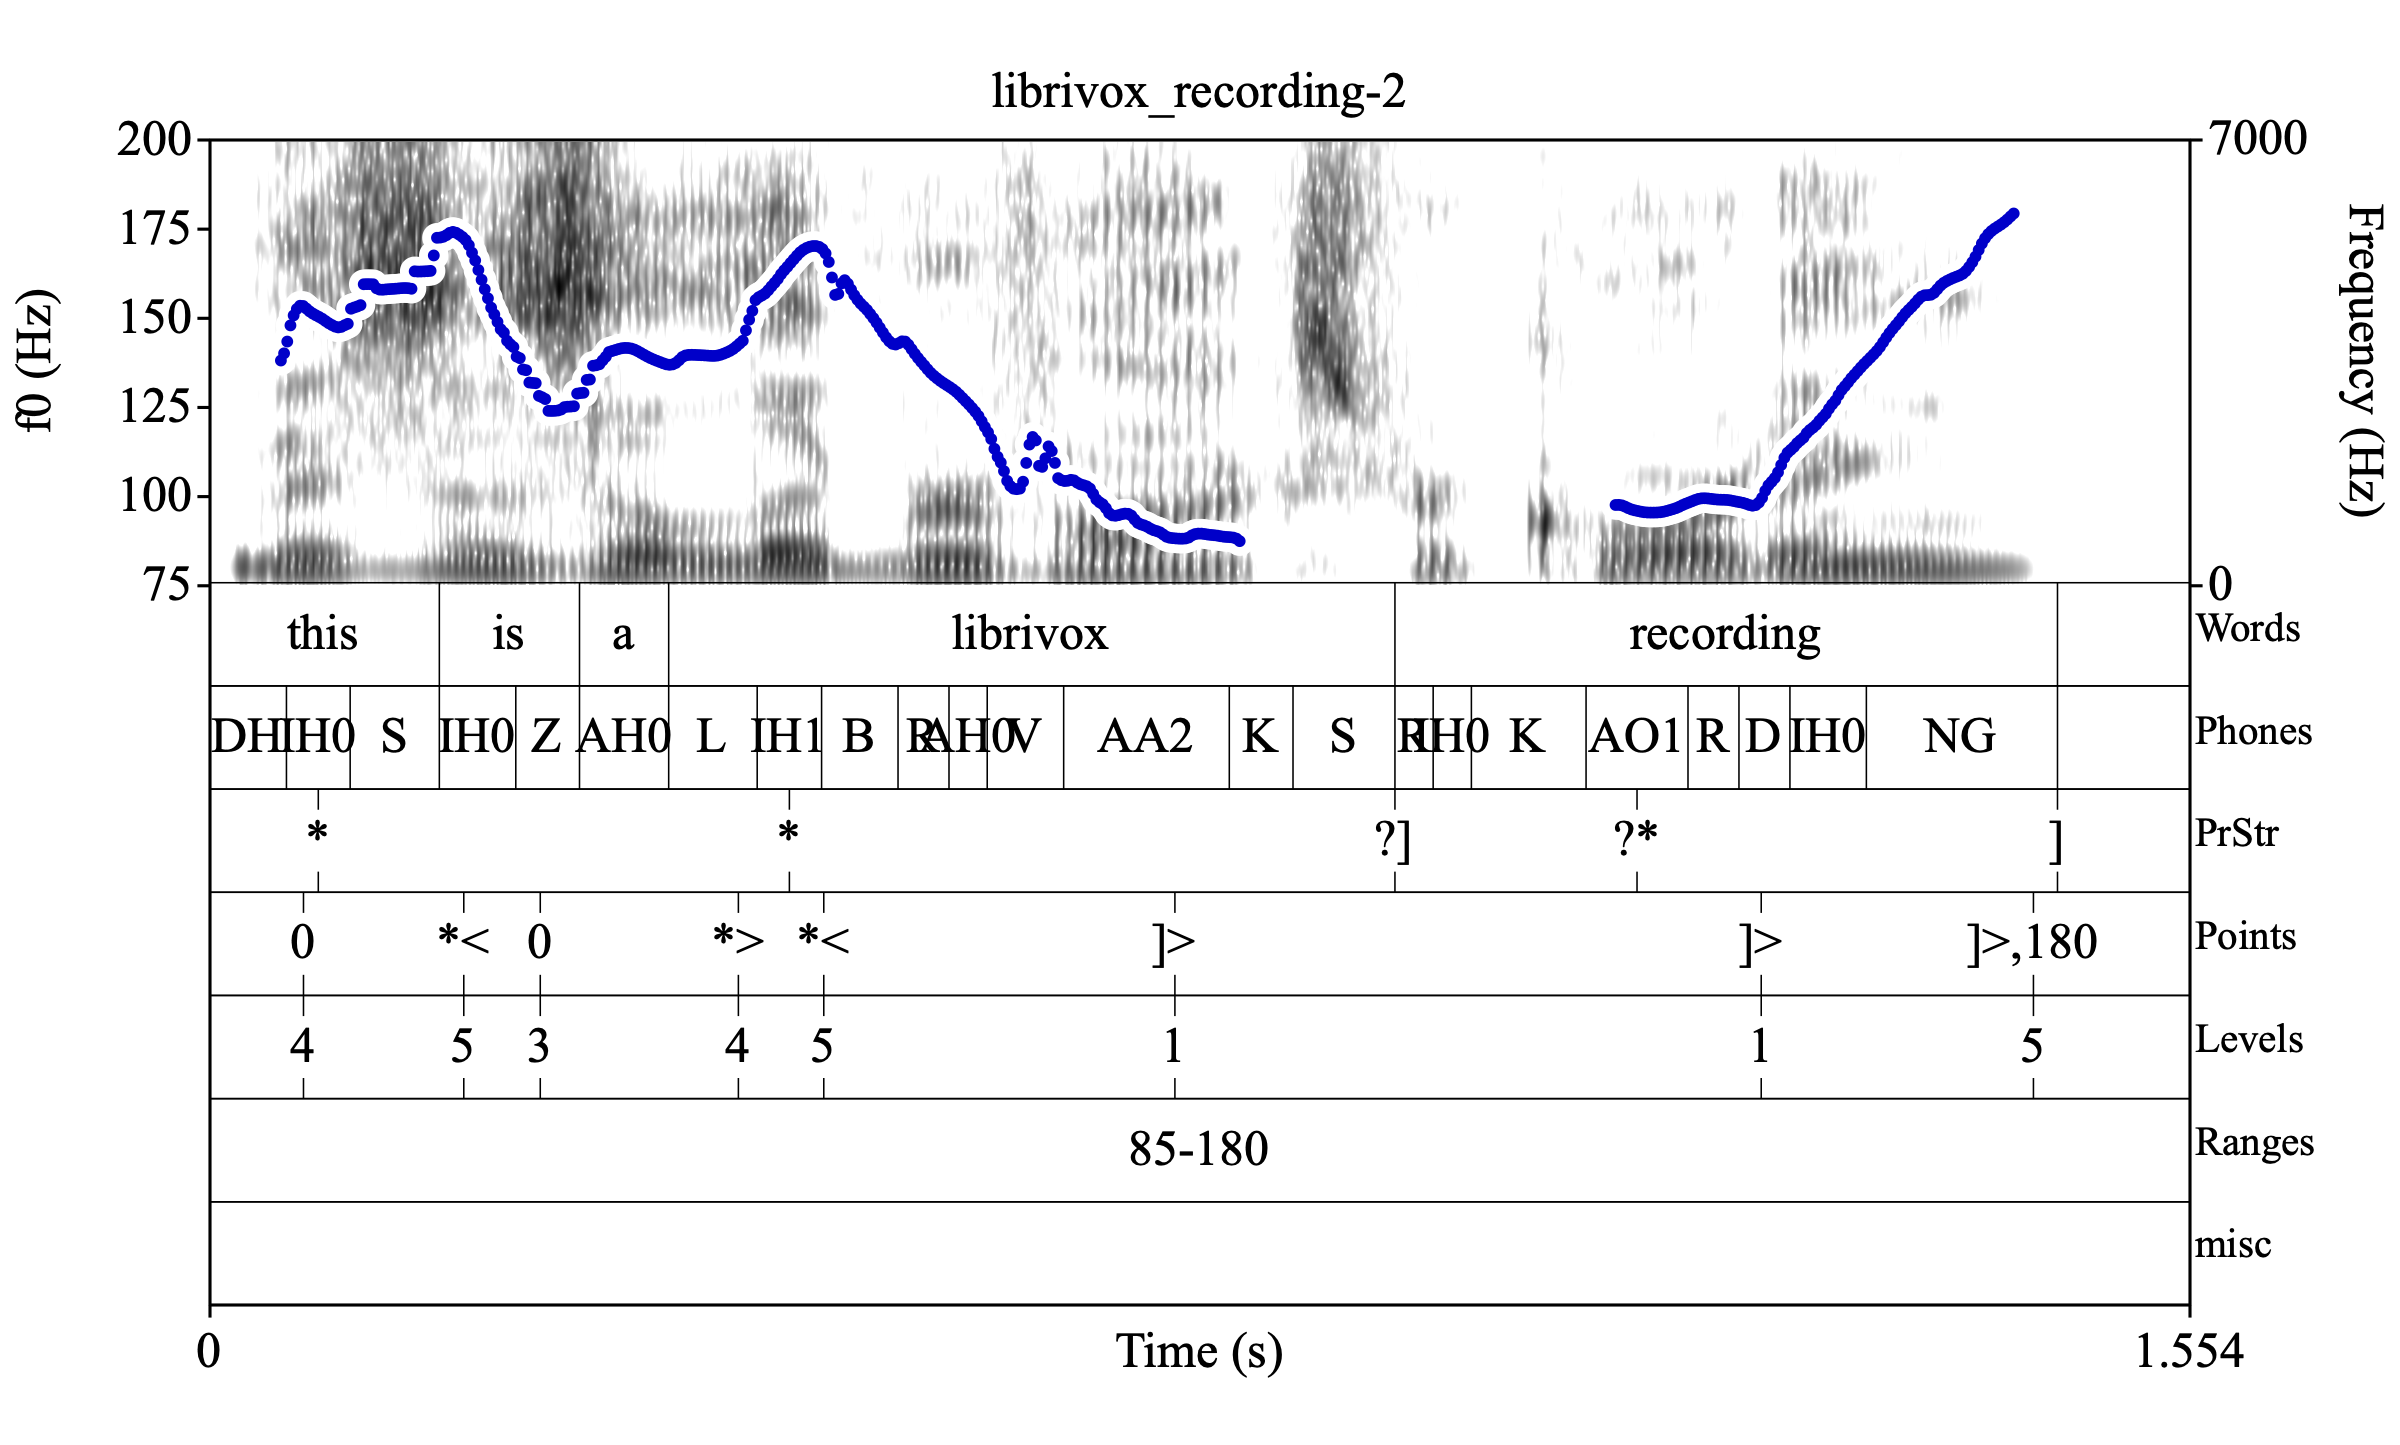
\includegraphics[width=.485\linewidth]{Usages-librivox_recording-2.png}
%
\caption{Two recordings of the same line by two speakers.%
\label{fig:Usages-librivox recording}%
\index{Annotated example, Usage cases!librivox\_recording-1}
\index{Annotated example, Usage cases!librivox\_recording-2}
}
\end{figure}

Here we see both speakers have Points tier labels associated with a \textlabel{*} on “\langtext{Librivox}”. Immediately we see the two are different in that the first speaker goes up two Levels (2-4) while the second only goes up one (4-5). At the same time, the latter has a slightly bigger local pitch range (95Hz) as compared to the former (75Hz). Comparing measurements based on these labels, we can also see that the Levels-based slope of the rise in the first one is slightly steeper (17.4 Levels/sec) than the rise in the second (14.9 Levels/sec), and that the peak in the latter is aligned earlier in the first example (towards the end of the stressed vowel interval) than in the second (just after the stressed vowel interval). These sorts of measurements could be calculated easily repeated across a large number of recordings, by making use of the “Extract info” functionality of the PoLaR plugin for Praat (see previous section) and using spreadsheet formulas or scripts for statistical analysis.

Let us return now to the idea of exploring variation in /\textlabel{L+H*}/ productions across different varieties. One issue that Burdin et al. faced (p.c.) is that the definitional boundaries of the \textlabel{L+H*} category that they appealed to were crafted for mainstream US English; as such, it is potentially problematic to use this label for these other varieties, when varieties can have mergers or splits with respect to categories (cf. variation in American English with respect to \langtext{caught}$\sim$\langtext{cot} or \langtext{merry}$\sim$\langtext{Mary}$\sim$\langtext{marry}). In other words: is it a problem to assume there is an \textlabel{L+H*} category that exists across varieties of English? And if so, how can we define the intonational form of that category so that it can be identified and compared across these varieties? To address this issue —which results from a top-down approach where a pre-established definition is used to pick out what should be acoustically compared— PoLaR labels can be used to define which intonational movements are similar enough to be compared. In other words, PoLaR labels (built from the bottom-up) can be used alongside some notions of what defines a category (e.g., a PrStr event and associated Levels values), in order to allow those elements that belong to the same category (according to those metrics) to be compared.



\begin{infobox}[frametitle=\textbf{Generating “Pseudo-Categorical” Labels from PoLaR Labels}]
	To be more concrete, we are advocating that “pseudo-categorical labels” (resembling A-M style categorical labels, like those used in systems like ToBI and IViE) can be created on the basis of PoLaR labels from the Phones, PrStr, Points, and Levels tiers, so long as the Points tier has Advanced labels. An example of such pseudo-categorical labels is given below (the third tier from the top, “Pseudo”, shows the these labels):
	
	\begin{minipage}{\linewidth}
	\begin{figure}[H]
	\centering
	%
	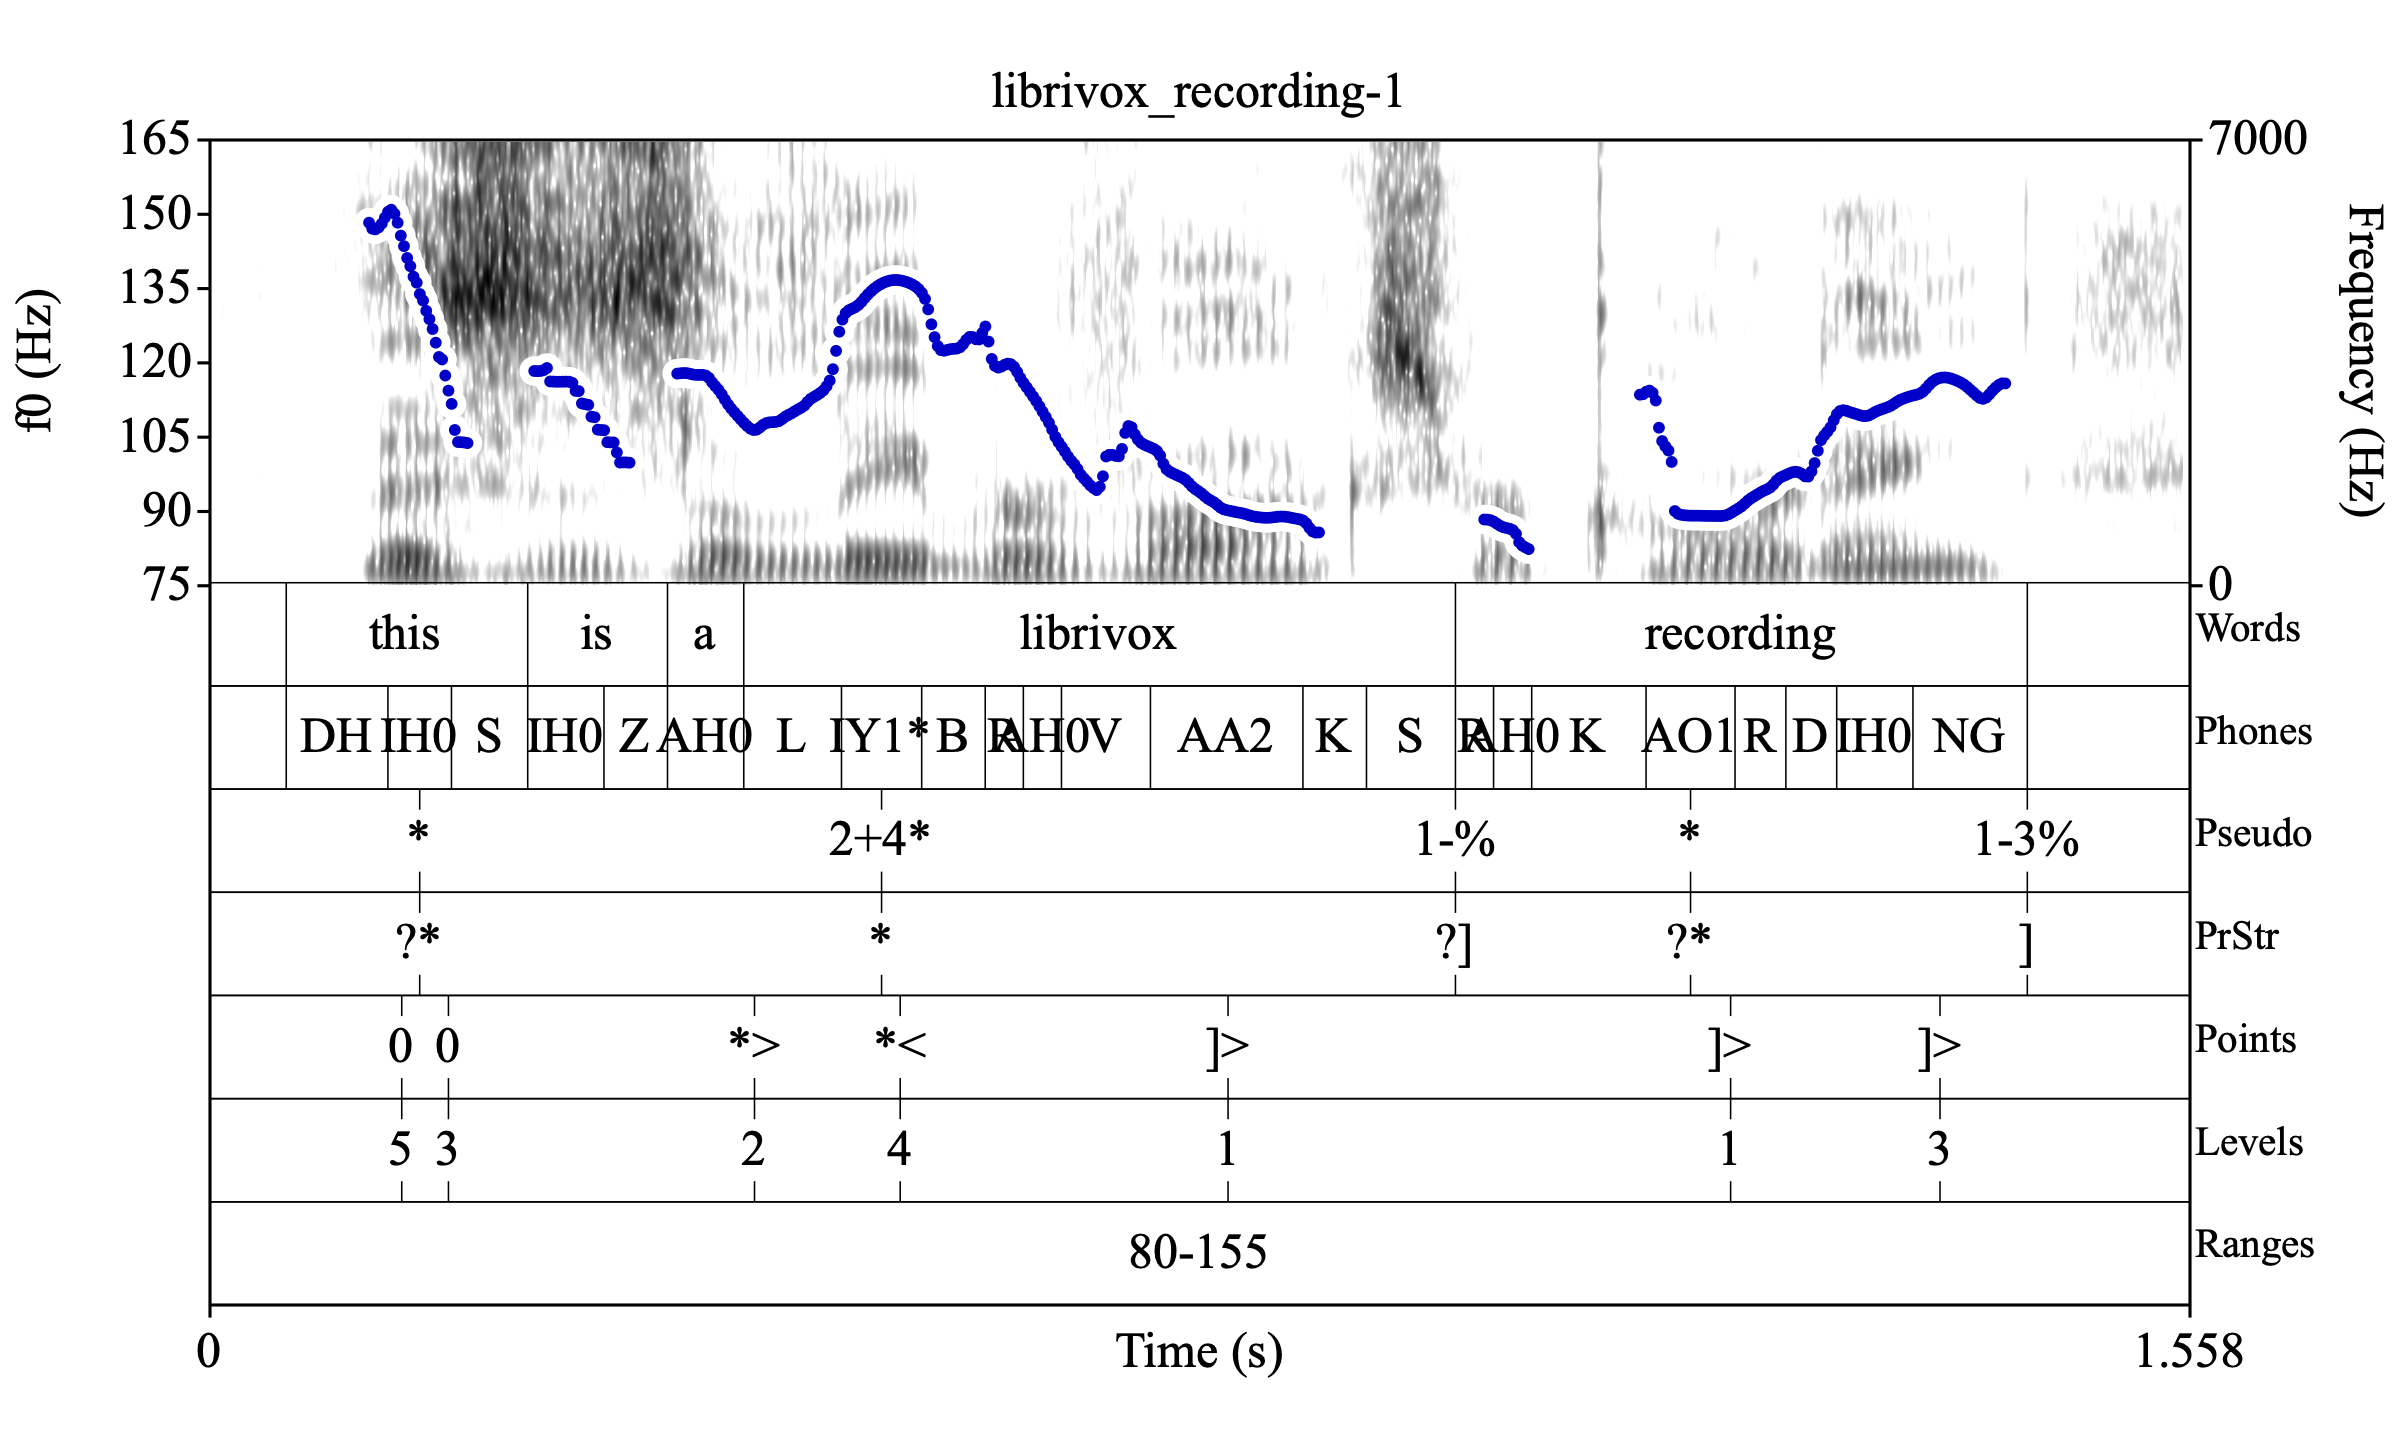
\includegraphics[width=.485\linewidth]{Usages-librivox_recording-1-pseudo-categorical.png} 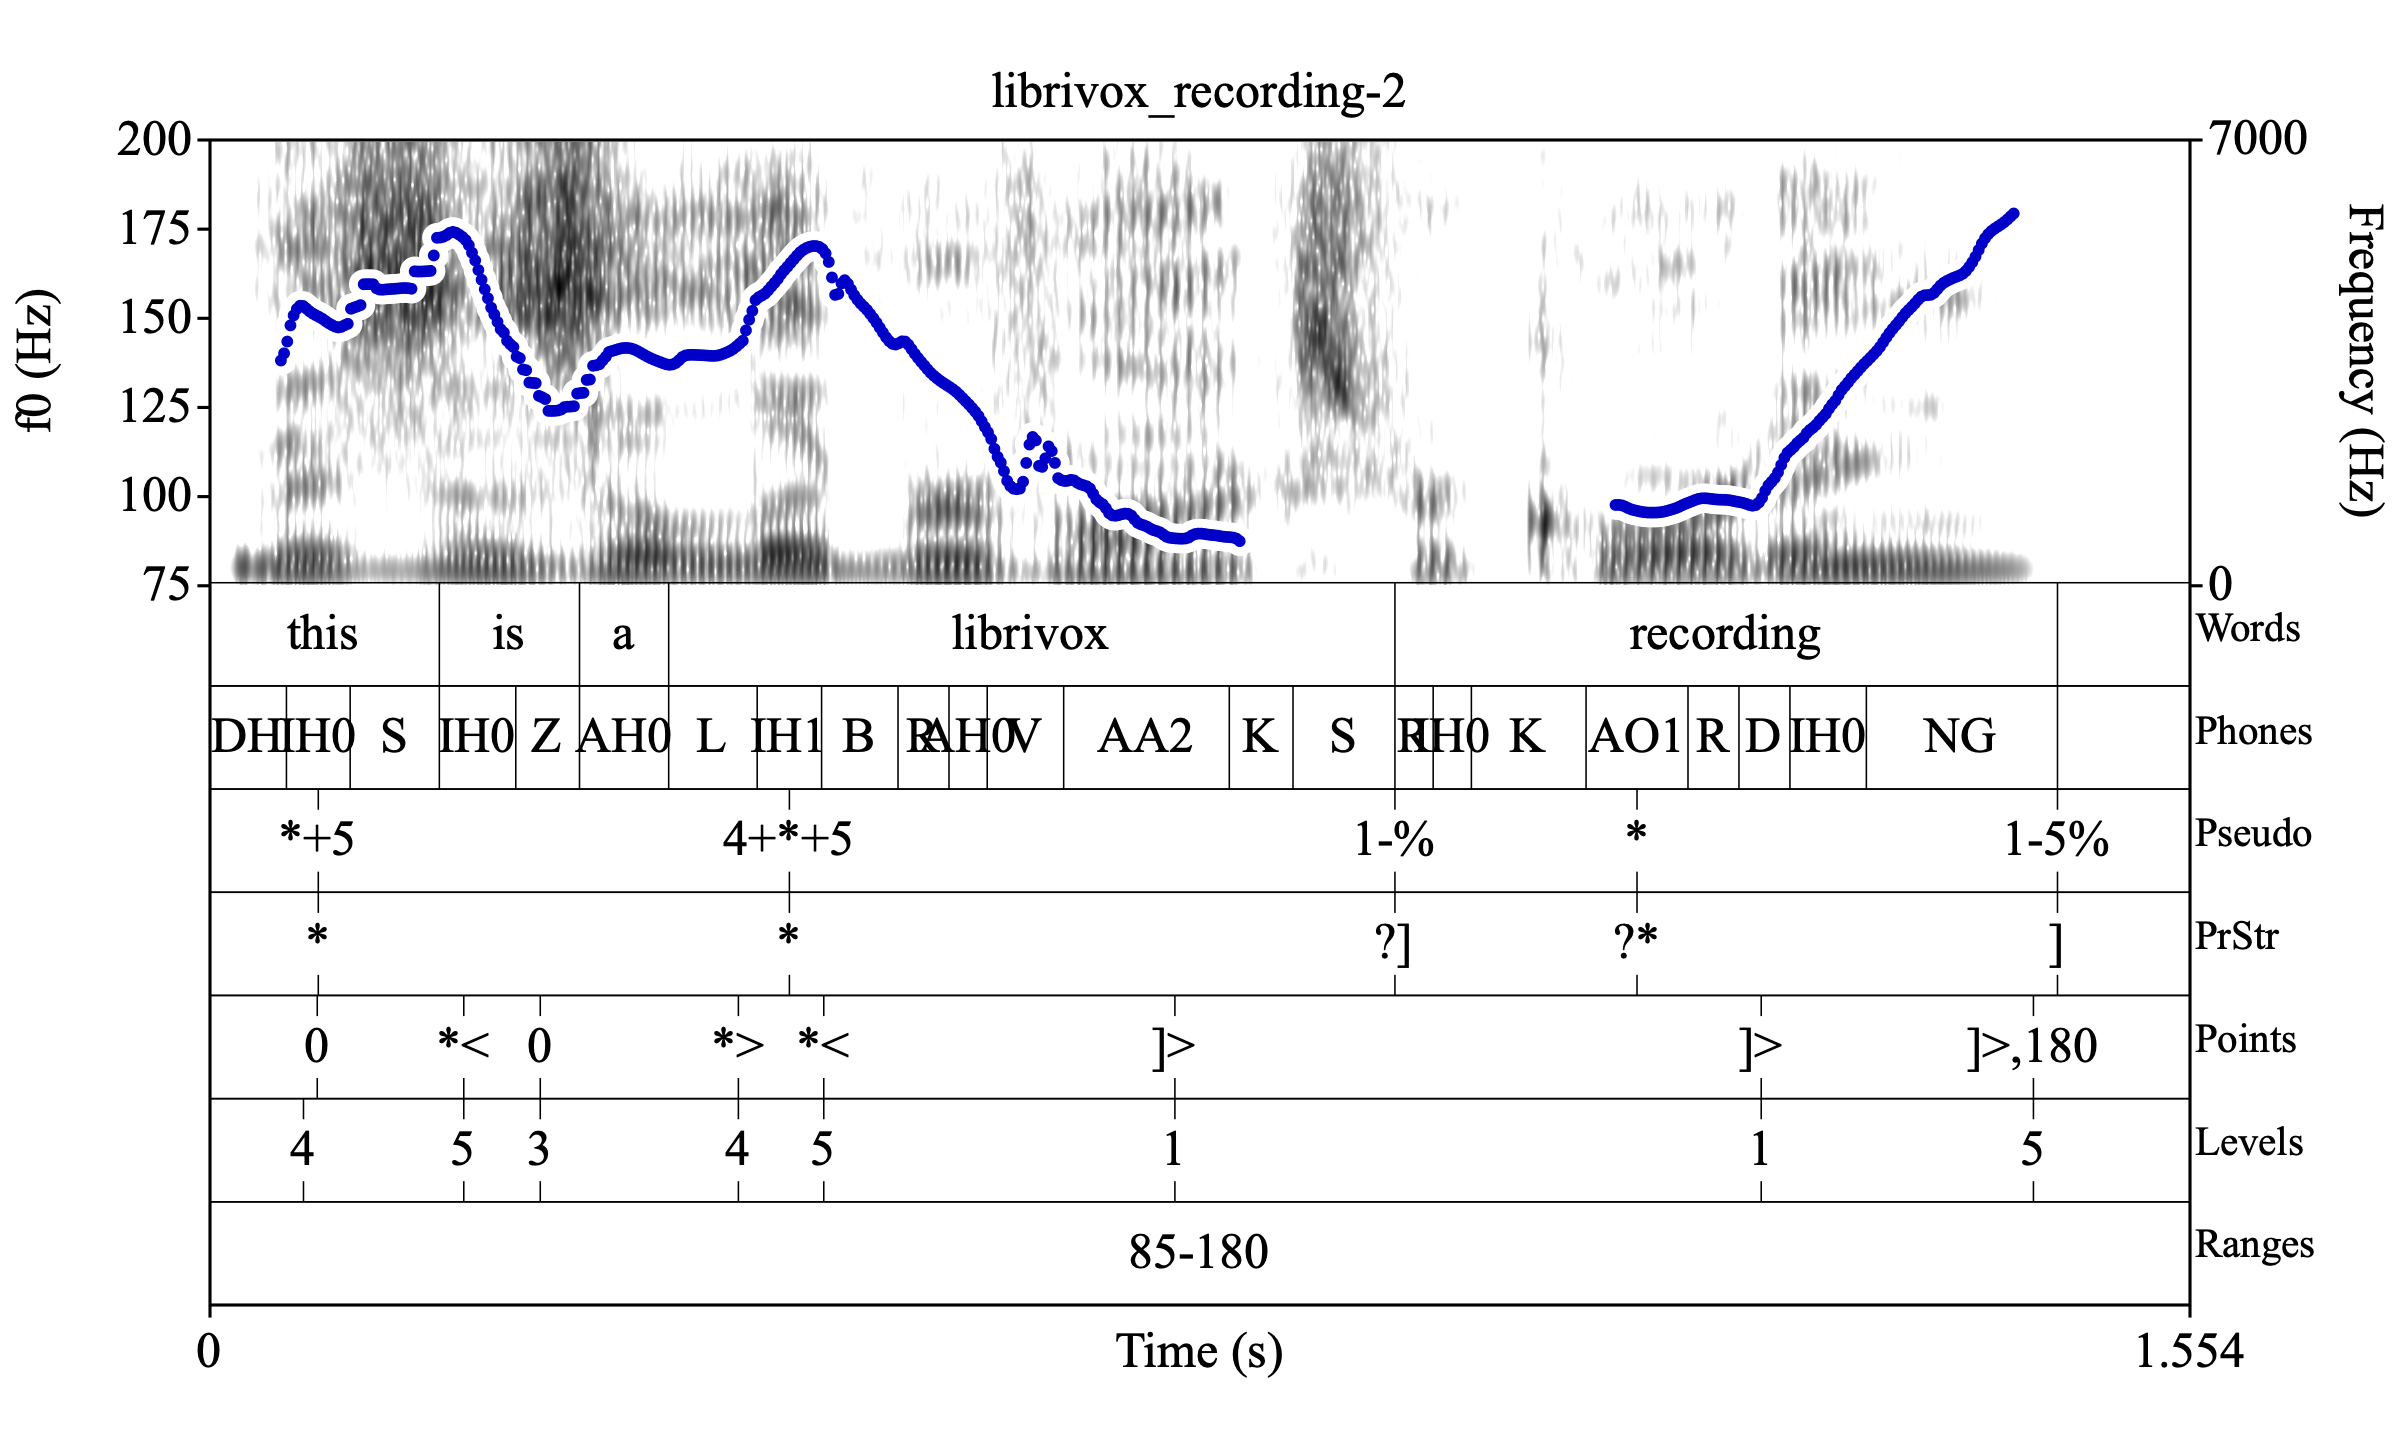
\includegraphics[width=.485\linewidth]{Usages-librivox_recording-2-pseudo-categorical.png}
	%
	\caption{Pseudo-categorical labels (3rd tier from the top) generated by a script in the Praat plugin, for \texttt{librivox\_recording-1} and \texttt{librivox\_recording-2}.%
	\label{fig:Usages-librivox recording pseudo categorical}%
	\index{Annotated example, Usage cases!librivox\_recording-2}
	}
	\end{figure}
	\end{minipage}

	Pseudo-categorical labels such as these can be especially useful in keeping track of the distribution of allophones, as described earlier in this section. In the examples above, assuming each instance of “librivox” is labelled /\textlabel{L+H*}/, we could say that /\textlabel{L+H*}/ has allophones of [\textlabel{2+4*}] and [\textlabel{4+*+5}].
	
	Of course using PoLaR labels to construct the boundaries of a category requires an algorithm. A preliminary attempt at implementing such an algorithm is coded into a script in the PoLaR plugin for Praat. The basics of this algorithm are as follows. We begin with prominence-associated labels. The script identifies the Phones-tier segments during which a \textlabel{*} label occurs and any Points tier labels that are associated with that \textlabel{*} (through \textlabel{<}, \textlabel{>}, or \textlabel{@} labels in the Advanced Points labels). For every \textlabel{*}-associated Points label within the relevant Phones interval, the corresponding Levels label appears next to the \textlabel{*} in the Pseudo tier label. For \textlabel{*}-associated Points labels that precede the relevant Phones interval, the associated Levels label(s) is/are inserted, followed by a \textlabel{+} (akin to ToBI complex tones). For example, during “\langtext{librivox}” in \texttt{librivox\_recording-1}, there is a \textlabel{2+4*} label indicating that the Level 4 Point occurs during the \textlabel{*}-marked segment, and it is preceded by a Level 2 Point that occurs before the \textlabel{*}-marked segment. On the other hand, in \texttt{librivox\_recording-2}, a \textlabel{4+*+5} label occurs within “\langtext{librivox}”, indicating that neither Points label occurs within the \textlabel{*}-marked Phone segment, and that a Level 4 Point occurs before the segment, and a Level 5 Point follows it. 

	As for boundary-associated labels, the script identifies the Phones-tier segments after which a \textlabel{]} label occurs and any Points tier labels that are associated with that \textlabel{]}. For every \textlabel{]}-associated Points label within or after the relevant Phones interval, the corresponding Levels label appears before the \textlabel{\%} in the Pseudo tier label. For \textlabel{]}-associated Points labels that precede the relevant Phones interval, the associated Levels label(s) is/are inserted, followed by a \textlabel{-} (akin to ToBI phrase accents). For example, after “\langtext{recording}” in \texttt{librivox\_recording-1}, there is a \textlabel{1-3\%} label indicating that the Level 3 Point occurs during the \textlabel{]}-marked segment, and it is preceded by a Level 1 Point that occurs before the \textlabel{]}-marked segment. After “\langtext{librivox}” in \texttt{librivox\_recording-1} there is a \textlabel{1-\%} label, indicating that there is a \textlabel{]}-associated Level 1 Point before the phrase-final segment, and no \textlabel{]}-associated Point during the phrase-final segment.

	Of course this algorithm is merely one attempt at transforming PoLaR labels into (pseudo-)categorical labels, and the nature of the algorithm must be revisited, as more is learned about the phonetics-phonology interface for intonation.
\end{infobox}

Finally, individual speakers within a dialect may also show systematic differences in their phonetic intonational habits, just as they do for cues to segmental features.  Given the increasing evidence that language users attend to and manipulate individual cues to phonological categories (and the values of those cues), it is likely to be fruitful to be able to capture these systematic patterns of variation for intonation.  Because PoLaR is tightly tied to observable events and values in the signal, and goes beyond the labelling of phonological categories to include phonetic values, it provides a tool for annotating such patterns.

While the discussion in this section is oriented towards exploring interspeaker variation within a language, similar methodologies can be used to build up a tonemic inventory for a language for which there has been little to no work on the intonational phonology.

\subsection{Patterns Related to Pitch Ranges}\label{sec:pitch-ranges}

Though it is well known that pitch range is dynamic —both over the course of a single utterance and across utterances— less is known about the more precise ways in which they change. Once more precise annotation is kept, we can ask ifDo the different ways in which pitch ranges change correspond to different (linguistic) contexts. There has been some research on the topic of pitch range and its connection to a variety of linguistic disciplines —including prosodic phonology, syntax, semantics, pragmatics, sociolinguistics, and discourse structure— from empirical angles of both production and perception.

As discussed in §\ref{sec:new-tier-range-changes}, PoLaR can be a useful tool for exploring the way that pitch ranges change. A core reason for this is that (as far as we know) no other intonational annotation systems beyond PoLaR requires explicit, systematic, and regular annotation of local pitch ranges and how they change. By including pitch range annotation as a core part of the labelling process, any PoLaR-labelled file can be used to investigate pitch range phenomena, even if that was not intended as a measurement for analysis by the original researchers who collected and/or labelled the data. Below we give a few examples of some research topics for which the Ranges labels could be used in analysis.

Below we give some examples of research that has yielded findings with respect to pitch ranges. After these paragraphs that provide an (abbreviated) overview of these topics, some abstract descriptions of ways in which PoLaR could be used to produce more nuanced results about pitch ranges will be provided. Finally, a sample recording is given with some more specific discussions about how PoLaR could be used to analyze the pitch range phenomenon.

In a variety of domains, there have been suggestions that changes in pitch ranges are tied to particular phenomena tied to linguistic meaning, broadly construed (e.g., semantically, pragmatically, and/or discourse structurally). This paragraph reviews one set of examples of pitch ranges ties to meaning, all from English. For example, yes/no questions have been found to have final rises that reach an extra high pitch, often higher than other highs in the utterance (cf. \citealt{pierrehumbert80}), suggesting that there is pitch range expansion that includes (at least) the final boundary movements. (Though perhaps the expanded pitch range applies to the entire utterance, as might be  suggested by the fact that initial f0 is higher at the beginning of a YNQ than a declarative; \citealt{sicoli-15}.) In addition, pitch ranges have been found to expand contexts expressing incredulity (\citealt{hirschbergward92}), surprisal\slash miriativity (\citealt{rett-20}), and emphasis\slash focus (\citealt{xuxu05}), or where the discourse topic shifts majorly (\citealt{hirschbergpierrehumbert86}). Beyond these examples of expansion, pitch range compression —systematically lowered pitch accent f0 peaks across phrases— has also been found to be associated with parentheticals (\citealt{price-91, dehe09}) with discourse coherence\slash continuation (\citealt{beckman93}, \citealt{bruce-97}). More broadly, a variety researchers have pointed to a role for pitch range relations in discourse segmentation, i.e. connecting phrases into coherent segments in discourses (\citealt{hirst93a}, \citealt{wichmann00}, \citealt{hirschberg04}, \citealt{lin-11}). Further research in these areas would benefit from PoLaR’s systematic labelling of pitch ranges.  Similar connections between pitch range and meaning has been found in a variety of languages – a small sample of such findings are in the domains of focus (Mandarin: \citealt{xu99}), parentheticals (French: \citealt{fagyal02}), discourse coherence (Swedish: \citealt{hansson03}, \citealt{carlson-05}).

In addition to these domains that are tied to particular meanings, questions oriented to phonological structure and syntactic structure can be asked too. It has been suggested that changes in f0 maxima for High pitch accents reflect hierarchical organization of prosodic phrases in multiple languages (\citealt{ladd88} for English, \citealt{fery-05} for German; \citealt{berg-92} for Dutch), and that such changes correspond to syntactic structure or cue grouping interpretation (\citealt{ladd88, ladd92}, \citealt{fery-05}, \citealt{kentnerfery13}), even when timing cues may be ambiguous or conflicting (\citealt{brugos15}). This direction of research relates to the question of the domain of downstepping, which has been said to be unable to apply across prosodic phrase boundaries in English (\citealt{beckmanayers97}); however, \citealt{sturman19} suggests such cross-phrase downstepping is possible with at least some types of prosodic phrases (large ones; in MAE\_ToBI terms: IP). Further research in this area is needed, and PoLaR is well suited to help, since Ranges are annotated completely separately from phrase boundaries.

As a final domain in which pitch range is explored, there are sociolinguistic and variationist findings tied to pitch ranges. For example, it has been suggested that African American English speech generally makes use of wider pitch ranges (marked by more falsetto and less downstepping; \citealt{wolfram-02, thomas07}), as compared to Mainstream US English. As another example, it has been found that newscasters and non-newscasters do not differ significantly in pitch ranges, but they do differ significantly in how much time is spent in different parts of their pitch ranges, and that this might be done as a way of encoding particular the conversational goals that newscasters have (\citealt{gasser-19}). PoLaR could again be useful to help keep track of not only Ranges (which could capture variation in usage of falsetto, downstep, and range size), but also Levels labels (which could capture how speakers make use of the same pitch range differently).

Let us turn now to the benefits of PoLaR for such explorations. Before proceeding, it must be mentioned that all the previously mentioned studies have achieved these results without PoLaR. While pitch range size can be tracked using directly observed f0 minima and f0 maxima, PoLaR provides a framework  dealing consistently with common pitfalls related to this (cf. §\ref{sec:intonational-contours-and-software-based-pitch-tracks} and §\ref{sec:some-trickier-cases-with-local-pitch-ranges}). Further, the PoLaR framework provides tools for analyzing range annotations with respect to the annotations of prosodic structure (on the PrStr tier), pitch movements (on the Points tier), and scaled pitch values (on the Levels tier). Further, as described in (§\ref{sec:new-tier-range-changes}), we can envision extensions to PoLaR to more directly associate Ranges tier labels to annotations of discourse or syntactic-pragmatic structure. 
%
\newline

In many works on pitch range (including in references above), researchers have defined expansion and compression by comparing the f0 height of pitch maxima across different utterances. However, since pitch ranges are defined by a ceiling and a floor, empirical questions remain about the pitch range changes. While findings have been established in relation to changes in pitch ceilings, less is known about the extent to which pitch floors and range span might play a role. One possibility is that different types of pitch range changes (compression from one\slash both ends, expansion at one\slash both ends, or shifts up\slash down) are associated with different types of linguistic contexts or communities of speech.

As a case in point about the value of tracking both the floor and ceiling of pitch range, \citet{dehewichmann10} write that “the typical parenthetical prosody is often, although not always, a marked shift to a compressed pitch range”. The same PoLaR labels that could be used to explore lowered f0 ceilings could also be used to explore the following questions: when do parenthetical pitch ranges compress\slash expand, compared to preceding range? How similar\slash different to each other are the ranges on either side of the parenthetical? Does the range ceiling ever get lower than the preceding range floor? Does the range floor ever get higher than the preceding range ceiling? While some of these variables can indeed be measured without PoLaR, it would require researchers to establish standards and conventions of their own. On the other hand, PoLaR labelling already includes this on the Ranges tier, and provides labellers with systematic annotation guidelines. Moreover, PoLaR allows labellers to make use of their intuitions with respect to labels, in a way that other direct measurements might not. 

Moreover, since it is known that pitch ranges are dynamic within an utterance, taking measurements of only pitch minima\slash maxima in an utterance restricts possible findings by preventing researchers from asking questions like how these pitch range changes are timed within an utterance (with respect to other prosodic events and/or particular words\slash morphemes). Labelling pitch ranges with PoLaR allows researchers to more directly address such questions via the greater detail about the magnitude and timing of range changes.  

Finally, using PoLaR could create hypotheses based on observed patterns in pitch ranges, or to check hypotheses about patterns in pitch ranges, with Ranges (and other PoLaR) labels defining what is measured. For example: one might explore whether the quantitative values of Ranges (with the min and max as continuous variables) are tied to particular parts of the utterance (e.g., timing with respect to word or phoneme boundaries, or relation to PrStr events). As another example: those interested in exploring how pitch ranges are used (e.g., how a speaker uses pitch within a range) could explore that through the Levels values of turning points in the pitch track and/or by calculating the area under the curve in different utterances, with the f0 or Levels values defining the curve (i.e., the ceiling) and the Range min defining the baseline (i.e., the floor). In both of these cases, as well as in others, users are encouraged to use the Extract Info functionality of the PoLaR plugin for Praat to extract the relevant measures into a spreadsheet-style format for easy analysis.

\subsection{Tonal Alignment and Tonal Center of Gravity}\label{sec:TCoG}
The alignment of the f0 contour over a prosodic event may cue various interesting aspects of spoken language. For example, the f0 alignment over the segmental string can be a cue to disambiguating the family of MAE\_ToBI categories \textlabel{L+H*} (late), \textlabel{H*}, \textlabel{H+!H*} (early) and \textlabel{L*+H} (late) often implemented in a rise-fall-rise context.  The alignment of a tonal event may also cue dialect distinctions or phonological allophones (that is, different f0 shape with same perceptual understanding).  Various measures of alignment have been proposed and used (e.g. with respect to the nucleus onset or center or with respect to an f0 peak or other turning points). Interesting results from these investigations (e.g. \citealt{niebuhr-11}, \citealt{dimperio00}) suggests that shape in concert with Turning Point alignment must also be considered.   

As an alternative to Turning Point based alignment, the Tonal Center of Gravity (cf. \citealt{barnes-10a, barnes-12}) is a global intonational measure that captures the perceptually salient aspects of alignment (TCoG-t) and scaling (TCoG-f). In the time domain, the TCoG-t is  the f0-weighted point in time. In the frequency domain, TCoG-f is the average f0 weighed by the intensity and recency with respect to f0 movements. Together, the TCoG values are global measures that capture the impact of  f0 turning points,  of f0 contour shape and of  the segmental\slash acoustic string on the perceived alignment of an f0 contour.  Thus the TCoG is a perceptually salient cue to f0 alignment and scaling, arguably more so than any (potentially missing) directly-measured f0 values such as peaks. 

Figure \ref{fig:TCoG} illustrates how the TCoG-t captures shape contributions in addition to the turning point locations. The TCoG (shown both in time and frequency here) varies even when the commonly-used rise-peak-fall turning points are held constant. As \citet{barnes-10a, barnes-12} have shown, these differences are perceptually salient, even when the precise point in time of the f0 is fixed.  

\begin{figure}[H]
\centering
%
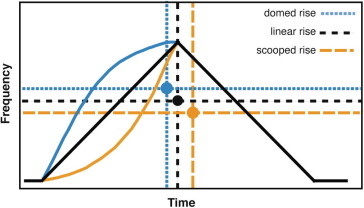
\includegraphics[width=.6\linewidth]{Usage-TCoG.png}
%
\caption{The gold dot indicates perceived alignment of rise-fall contour when rise is scooped, while the blue dot indicates perceived alignment when rise is domed. These shape changes influence the perceived alignment even though the turning point remains constant.%
\label{fig:TCoG}%
%\index{Annotated example, Usage cases!XXX}
}
\end{figure}

As an average over many f0 values, the TCoG can furthermore be modeled to incorporate the impact of changes in f0 salience over differences in intensity and/or sonority by including weighting factors.  It has been suggested that F0 perception is strengthened\slash more salient over areas of greater periodic energy (\citealt{albert-18}), greater sonority (\citealt{barnes-14}), and/or at the end of  pitch movements (\citealt{dalessandro-95}). 

However, once one concedes the need to account for both f0 shape and alignment over the segmental string, there is  still the open research question concerning the bounds of the salient interval. Specifically, over what interval is the weighted f0 averaged?  Two obvious candidates are (a) the segmental domain (related to the accented vowel\slash syllable) or (b) the intonational domain (related to deliberate prosodic event related f0 movements) although it is possible that listeners integrate both.

In resynthesized laboratory stimuli adjusted to explore alignments, the segmental and f0 turning point domains often are designed so that they overlap substantially.  Furthermore, these stimuli do not take into account accommodations speakers might make to adjust to a segmental string (e.g., earlier or later f0 movements around unvoiced regions or avoiding pitch movements on non-accented syllables). However, using naturally occurring speech presents difficulties in calculating f0 values.

For example,  (as mentioned extensively throughout this guide) human speech typically does not result in smooth and continuous f0 contours with clearly discernible turning points.  In fact, turning points can be missing even during intervals thought to be the most important phonologically (e.g., peaks of High accents). For example, f0 points may be missing at critical locations due to a voiceless sound source, or the f0 track may take the form of a plateau.  PoLaR provides two ways of capturing this missing information: 

\begin{enumerate}
	\item Annotators can use the “comma-override” in the Points tier to estimate the missing f0 values in crucial locations.
	\item Annotators can place inflection points (i.e. in the dome or scoop elbow) in the Points tier to create distinct straight line approximations of the perceived f0, presumably adjusting the contour to align in the same way the TCoG does.
\end{enumerate}

PoLaR labeling could be useful in providing data to investigate alignment and scaling behavior by allowing researchers to examine the TCoG in unconstrained (rather than laboratory) speech. Naturally occurring, unscripted speech carries variation in f0, the quality of the f0 contour, and the energy in segmental implementation which can provide variety to investigate accommodations that speakers make to preserve the meaningful prosodic cues.  Using PoLaR labels would therefore enable automation of the TCoG calculations over large corpora, to explore the TCoG in utterances produced “in the wild”. This, in turn, could allow researchers to explore alignment and scaling in a larger variety of contexts. 


\section{Issues in Labelling Minimized by PoLaR’s Design}\label{sec:logistical-issues-in-labelling}

In addition to facilitating work on research questions about intonation in new ways, PoLaR’s design should minimize some common issues that arise in using existing intonational annotation systems (especially those that are categorical). In this section, we break down these issues into two fundamentally different types: those that are process-oriented (e.g., relating to disagreements and uncertainty) and those that are theory-oriented (e.g., relating to poorly understood and/or understudied intonational phenomena).

\subsection{Disagreements and Uncertainty Minimized by PoLaR’s Design}\label{sec:reducing-inter-labeller-disagreement}

As mentioned elsewhere in this monograph, PoLaR labels on different tiers are largely independent of one another, a design feature which has the potential to (i) facilitate labelling, (ii) significantly reduce labeller disagreements (e.g.  by reducing both subjectivity and uncertainty), and (iii) guide discussion toward resolution of problems and new analyses. The independence of different tiers means that the labeller can deal with one tier at a time, and it is easier to learn how to label one tier than to master labels that bundle a variety of intonational characteristics together.  Thus the independence of the tiers provides a low barrier to entry for novices. It also means that the overall labelling task can be divided among multiple labellers working in parallel on different tiers.

In addition to disagreements that may arise from bundled labelling, labelling discomfort sometimes arises because of uncertainty.  To increase labeller confidence, PoLaR provides tools that can be used to check a candidate label.  For example, the Straight Line Approximation tool provides a convenient mechanism for checking whether a particular Points label is required or not, and the Levels labeller tool can be used to check Ranges labels.  Because PoLaR labels map relatively transparently onto signal characteristics, many aspects of labelling are quite mechanical (and for some aspects, fully automatic); this reduces uncertainty (and thus, disagreement). An exception to this is the categorical labels (i.e. PrStr labels), which are still quite abstract and require listener judgments. In the future, one way to avoid disagreements might be to source these labels from RPT (thereby replacing potential disagreements in categorical labels with crowdsourced labels serving as a kind of consensus label, and offering the additional benefit of capturing the degree of ambiguity perceived by a group of listeners). 

Another advantage provided by the design of PoLaR is the separation between Basic labelling (which focuses on prosodically relevant acoustic characteristics and requires no or minimal interpretation) and Advanced labelling (which permits the labeller to add more details in a second pass, including more interpretive notations). The flexibility of the system also allows experienced labellers and researchers who are interested in particular aspects of the intonational signal to easily add relevant labelling tiers.  These design features (separation and flexibility) have the potential to provide good agreement on the more transparent Basic labels, and to restrict disagreement to the Advanced labels, where the discussion may be more fruitful.  We note that PoLaR focuses largely on cues rather than on the contrastive categories of intonational phonology; as a result, the fact that different speakers and listeners (and labellers) may interpret cues to phonological categories differently becomes less of a problem.  The mapping between cues and phonological labels, which may be complex, is left for further analysis and discussion, while the annotation of the cues themselves may be more straightforward and less subject to disagreement.

To exemplify how PoLaR can reduce labeller disagreements and facilitate focused discussion, here we consider some examples of disagreements that often arise in alternative labelling systems that are designed for phonological labelling (e.g., MAE\_ToBI), and consider how working with PoLaR might help. When such a case arises, the labels themselves direct labellers to specific aspects of the signal to discuss. For example, consider the utterance below, where labellers disagree about whether the high pitch during “it” ought to be labelled as \textlabel{H*}, as \textlabel{\%H}, or not labelled at all.

\begin{figure}[H]
\centering
%
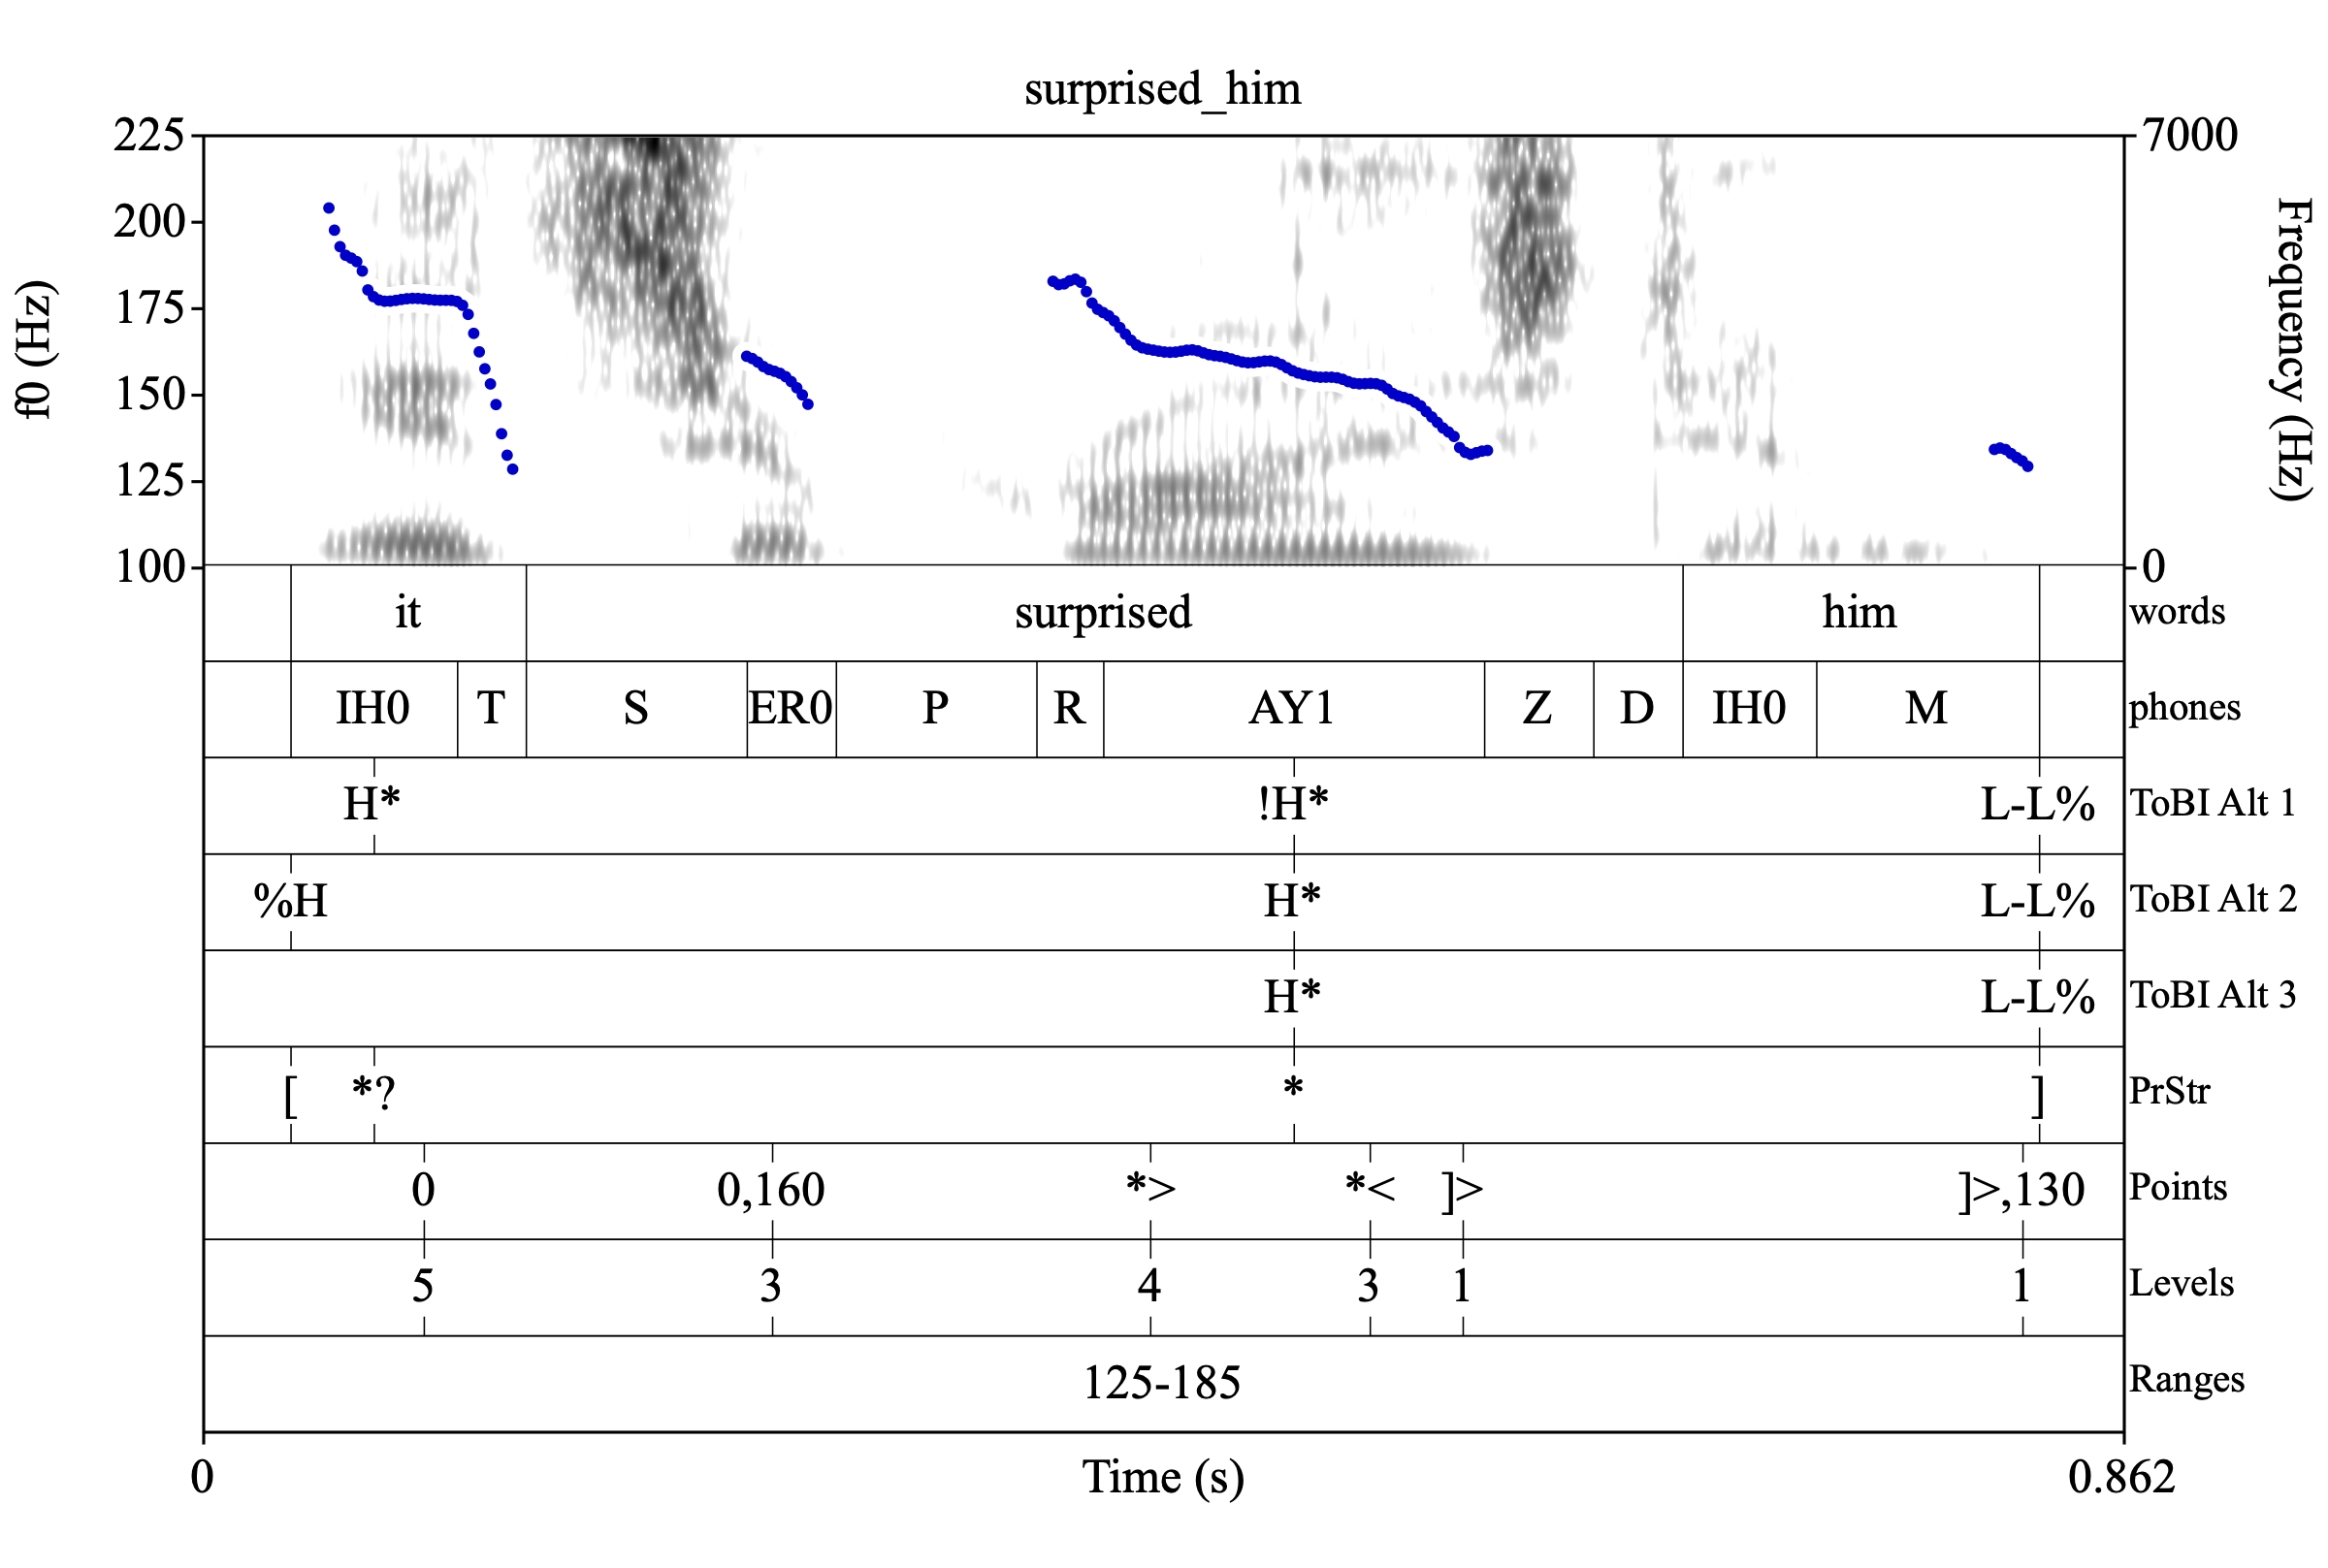
\includegraphics[width=.875\linewidth]{Usages-surprised_him.png}
%
\caption{MAE\_ToBI labellers may disagree or be uncertain about whether what’s most appropriate for the initial high pitch is a \textlabel{H*} label, a \textlabel{\%H} label, or no label at all. The different possible labels are indicated on the three “ToBI Alt” tiers.%
\label{fig:Usages surprised him}%
\index{Annotated example, Usage cases!surprised\_him}
}
\end{figure}

Is this because of different perceptions with respect to prominence (i.e., \textlabel{H*} vs. \textlabel{\%H} or no label), or is it because labellers disagree whether the pitch is meaningfully at a high target (i.e., \textlabel{H*} or \textlabel{\%H} vs. no label)? Instead of forcing annotators to choose an analysis before creating a complete set of labels, PoLaR allows the uncertainty of prominence to be captured as a \textlabel{*?} on the PrStr tier, and the lack of commitment to a specific phonological analysis is captured as a \textlabel{0} on the Points tier. For labellers who are more certain, the source of perceptual\slash analytical differences will be easier to identify and discuss, with PoLaR labels that pull apart the relevant issues. In this specific case, the perceptual issue of prominence will be clear through PrStr labels for “\langtext{it}” (i.e., \textlabel{*} vs. \textlabel{*?} vs. nothing), and the analytical issues can be captured as Advanced Points labels (i.e., \textlabel{<[} vs. \textlabel{<*} vs. \textlabel{0}).

As a second example, labellers quite commonly disagree over —or are uncertain about— whether a particular label ought to be \textlabel{L+H*} or \textlabel{H*}, as below.

\begin{figure}[H]
\centering
%
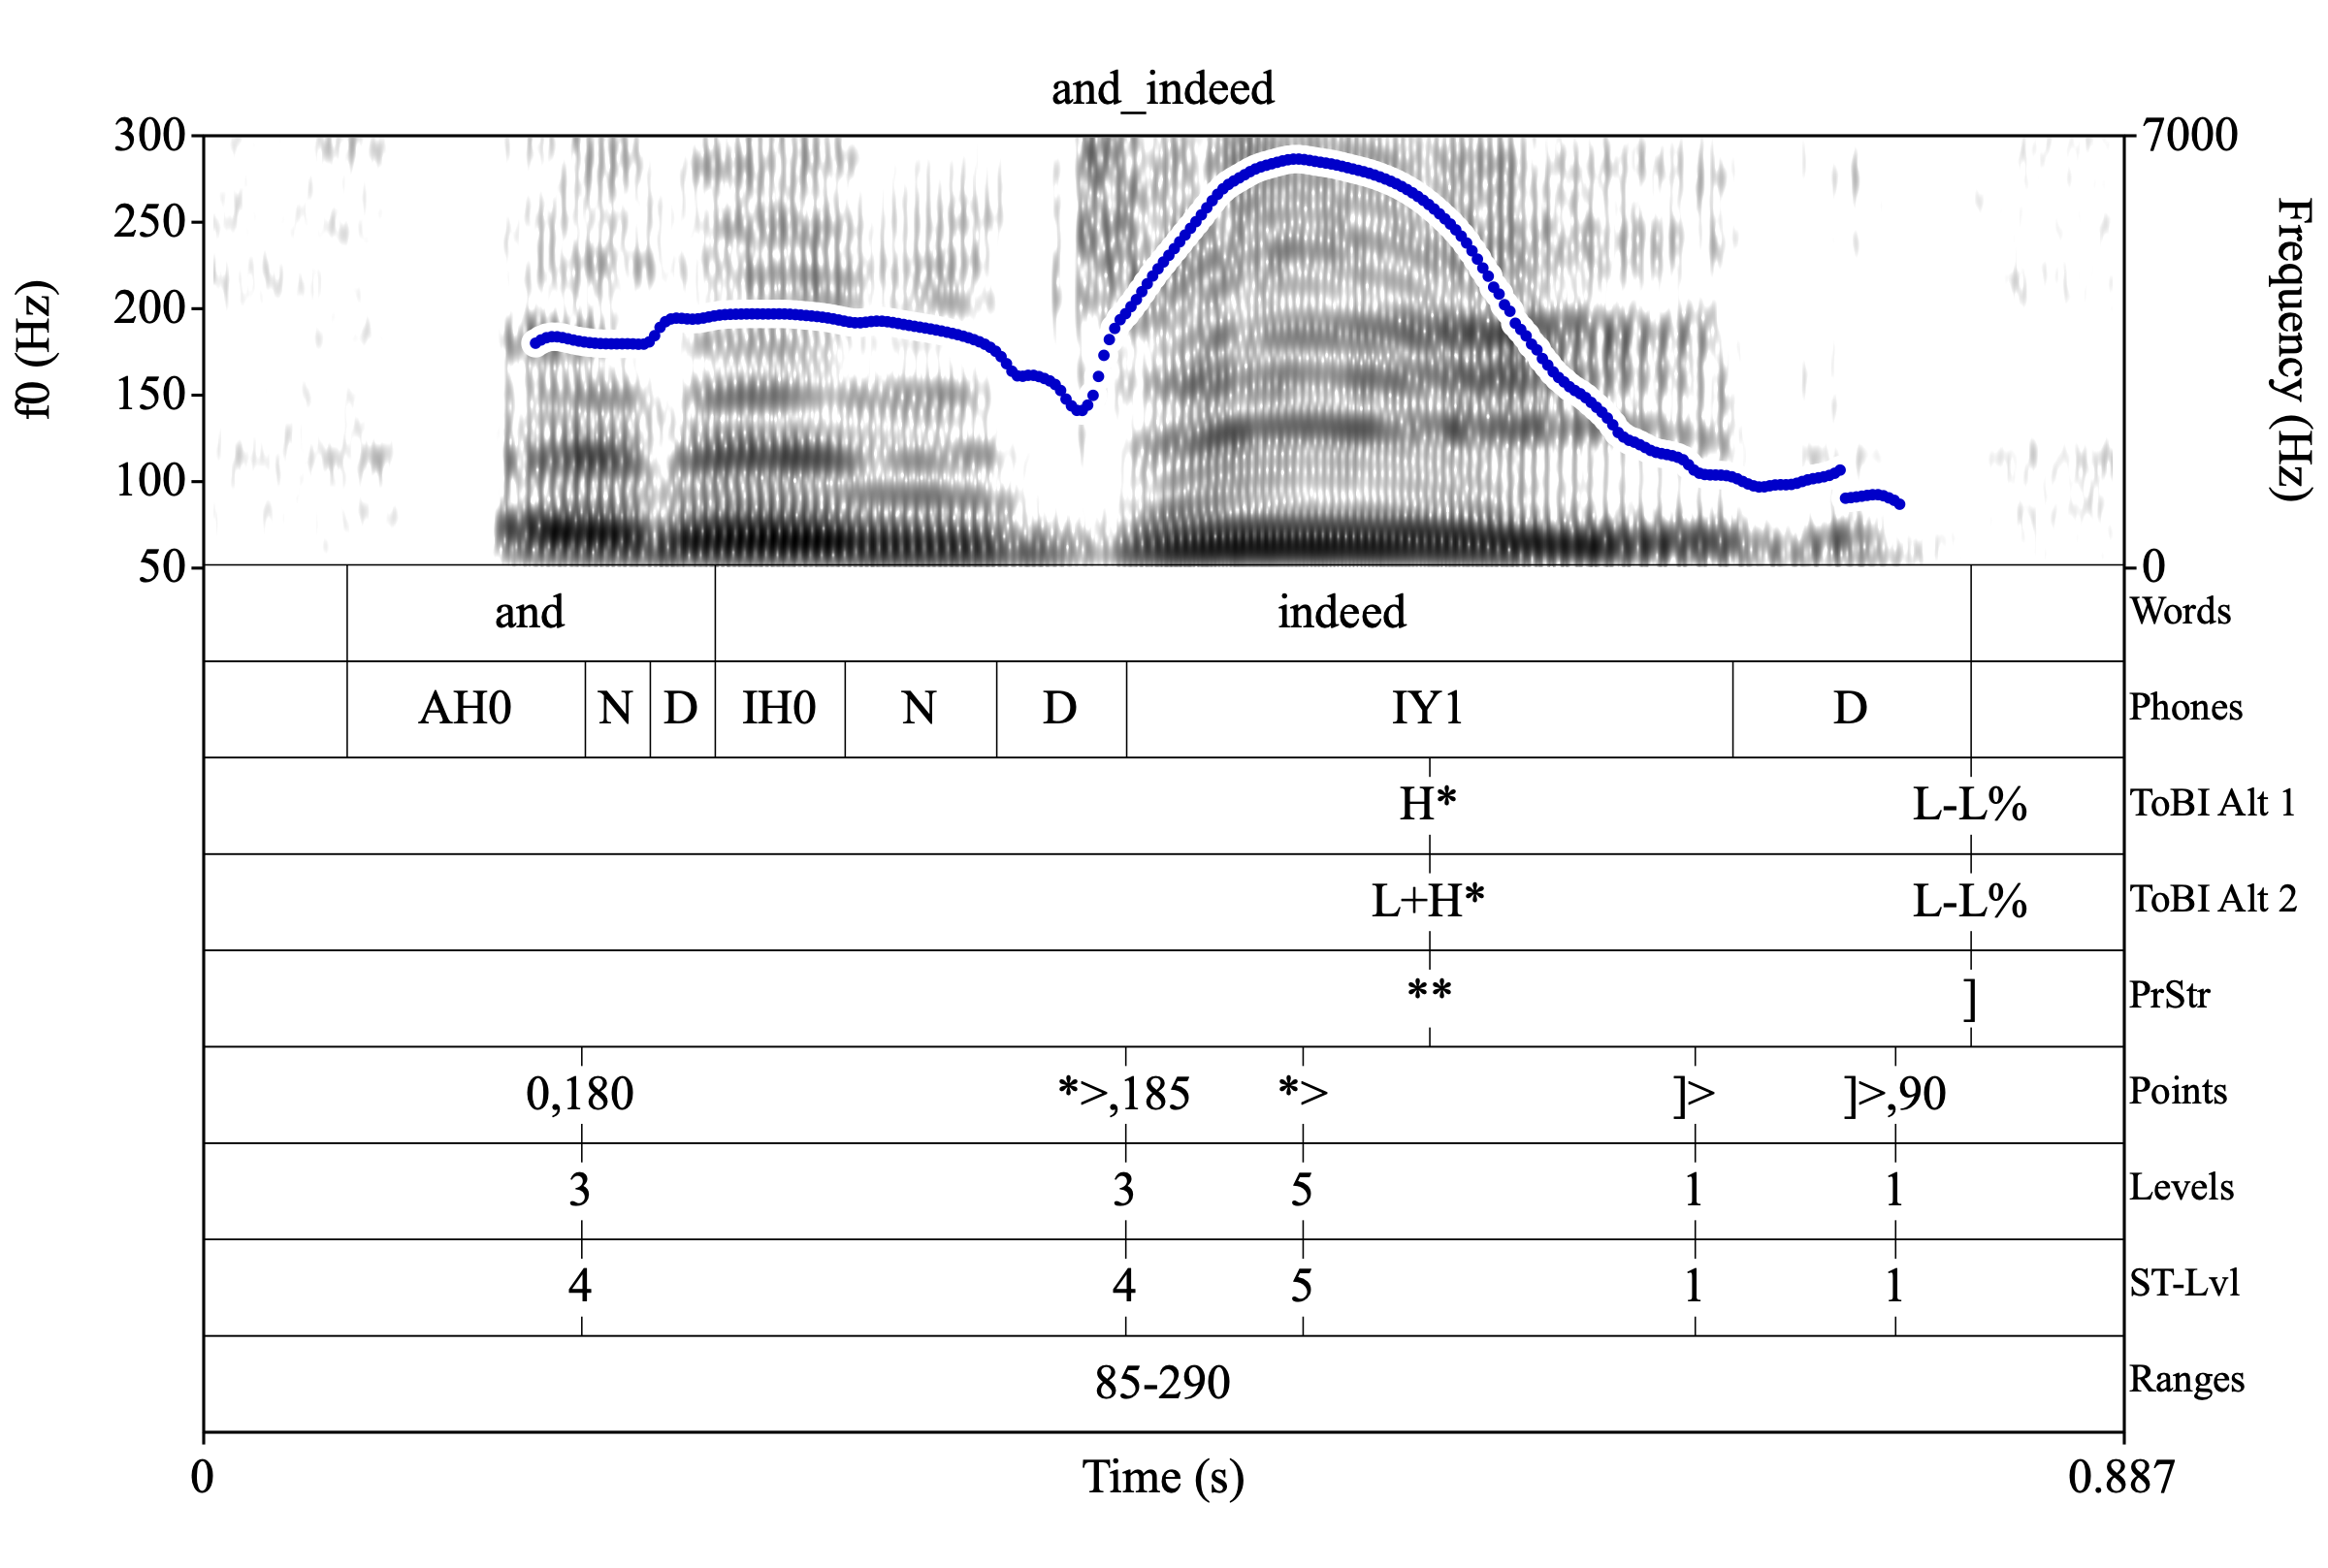
\includegraphics[width=.875\linewidth]{Usages-and_indeed.png}
%
\caption{MAE\_ToBI labellers may disagree or be uncertain about whether a label of \textlabel{L+H*} or \textlabel{H*} is more appropriate for “\langtext{indeed}”. The different possible labels are indicated on the two “ToBI Alt” tiers.%
\label{fig:Usages and indeed}%
\index{Annotated example, Usage cases!and\_indeed}
}
\end{figure}

This disagreement or uncertainty in phonological labels may be because the labellers have different criteria for what constitutes an \textlabel{H*} vs. \textlabel{L+H*}, or it could be that they differ in their perception of which phonological category is expressed, or both. On the other hand, because Points and PrStr are labelled separately, the PoLaR labels can indicate which aspects of the signal were perceived differently by different labellers. For example, in Figure \ref{fig:Usages and indeed}, this PoLaR labeller analyzes the lower f0 at the beginning of the vowel as associated with the prominence (using the Advanced \textlabel{*>} label on the Points tier), but another labeller might leave this as a \textlabel{0} label indicating they are not analyzing it as associated with the prominence. This information will be useful in focusing discussions about which phonological label (if any) is most appropriate.

In sum, PoLaR labels can lead to more fruitful discussions about how aspects of the signal map onto categorical labels, making it possible to identify some of the issues with categorical labels related to how different labellers interpret the signal differently (unbeknownst to themselves and/or each other). In addition, if PoLaR labellers want to include MAE\_ToBI labelling, the PoLaR labels can be used as a guide.  For example, a decision could be made about which labels ought to be \textlabel{H*} and which should be \textlabel{L+H*}, e.g., by following an algorithm based on the time-alignment of Points with respect to syllable boundaries, and/or pitch-scaling of Levels.


\subsection{Unlabellable Cases Minimized by PoLaR’s Design}\label{sec:difficultunlabellable-cases}
One of the goals of (phonological) grammars is to predict what sorts of expressions are possible and which are impossible. Being able to accurately make such predictions is the marker of a successful phonological analysis, and many prosodists and intonationists have the goal of understanding where the boundaries of well-formedness lie, and thus make proposals to that end. Some of these proposals constrain systems of prosodic annotation, sometimes to the extent that the annotation system is unable to transcribe a signal that does not conform to the proposed grammar. This issue —the existence of what we call “unlabellable” cases— is one that such systems cannot be used to address, without serious modification.

On the other hand, PoLaR is not tied to any particular phonological grammar, and thus there are no unlabellable cases. Though there are no unlabellable utterances, there is a system for annotation that a researcher can use to describe these otherwise-unlabellable utterances. The benefits of this are rather clear, and below we provide a few examples of cases where PoLaR can be used where other phonologically-tied annotation systems cannot be.

As a first example, in exploratory studies on un(der)documented languages and varieties, most or all utterances are “unlabellable” in the sense that one would need some sort of prosodic theory of the language\slash variety to start using a phonologically-defined labelling system. In many cases, using an existing annotation system may not be appropriate (because of grammatical dissimilarity among the languages\slash varieties), and creation of a new phonological annotation system may not be immediately feasible. PoLaR might be particularly useful in such cases, to aid in finding describable and analyzable patterns. As noted above, for many PoLaR labels (especially Basic labels), minimally-trained annotators can systematically label essential aspects of prosody, even if they are not a speaker of the language\slash variety being studied. For the PoLaR labels that do require speaker intuitions (e.g., PrStr labels), researchers could use experimental methodologies (such as RPT tasks) to crowdsource judgments from speakers of the language.

After PoLaR-annotating speech data from such languages\slash varieties, researchers in developing phonological analyses can use the patterns in their PoLaR labels to identify aspects of the signal that signal different prosodic categories (e.g., shapes defined by Points\slash Levels labels that are timed with respect to PrStr labels). For example, \citet{kapia-19} and \citet{brugos-21} have begun to use this methodological division of labor in the exploration of the intonation of Albanian, with PrStr tier annotations informed by both RPT from naïve native speakers and by a trained native speaker of Albanian, and aspects of acoustic phonetic prosody (Points and Ranges) being annotated by a trained labeller who is not a speaker of the language.

In addition to the cases that are “unlabellable” because no phonological labelling system exists (i.e., in early investigations of languages\slash varieties), phonological labelling systems (by design) also limit what is labellable to utterances whose forms are predicted to by possible by the grammar of the labelling system. In other words, if a phonological labelling system is in any way incomplete or inaccurate in the boundaries it sets for what is prosodically (im)possible, there will necessarily be utterances that are “unlabellable”. (In addition, because some cases are indeed unlabellable, a researcher may find themselves wondering about particular (challenging) examples “\textit{Does this conform to the grammar in my theory, and if I’m not sure, which labels should I use?}”. This can lead to issues of uncertainty or disagreements about labels, of the sort described in the previous section.)

As a concrete example of utterances that are “unlabellable” because their prosodic properties are not predicted possible by the grammar, consider the mainstream U.S. English yes/no questions below:

\begin{figure}[H]
\centering
%
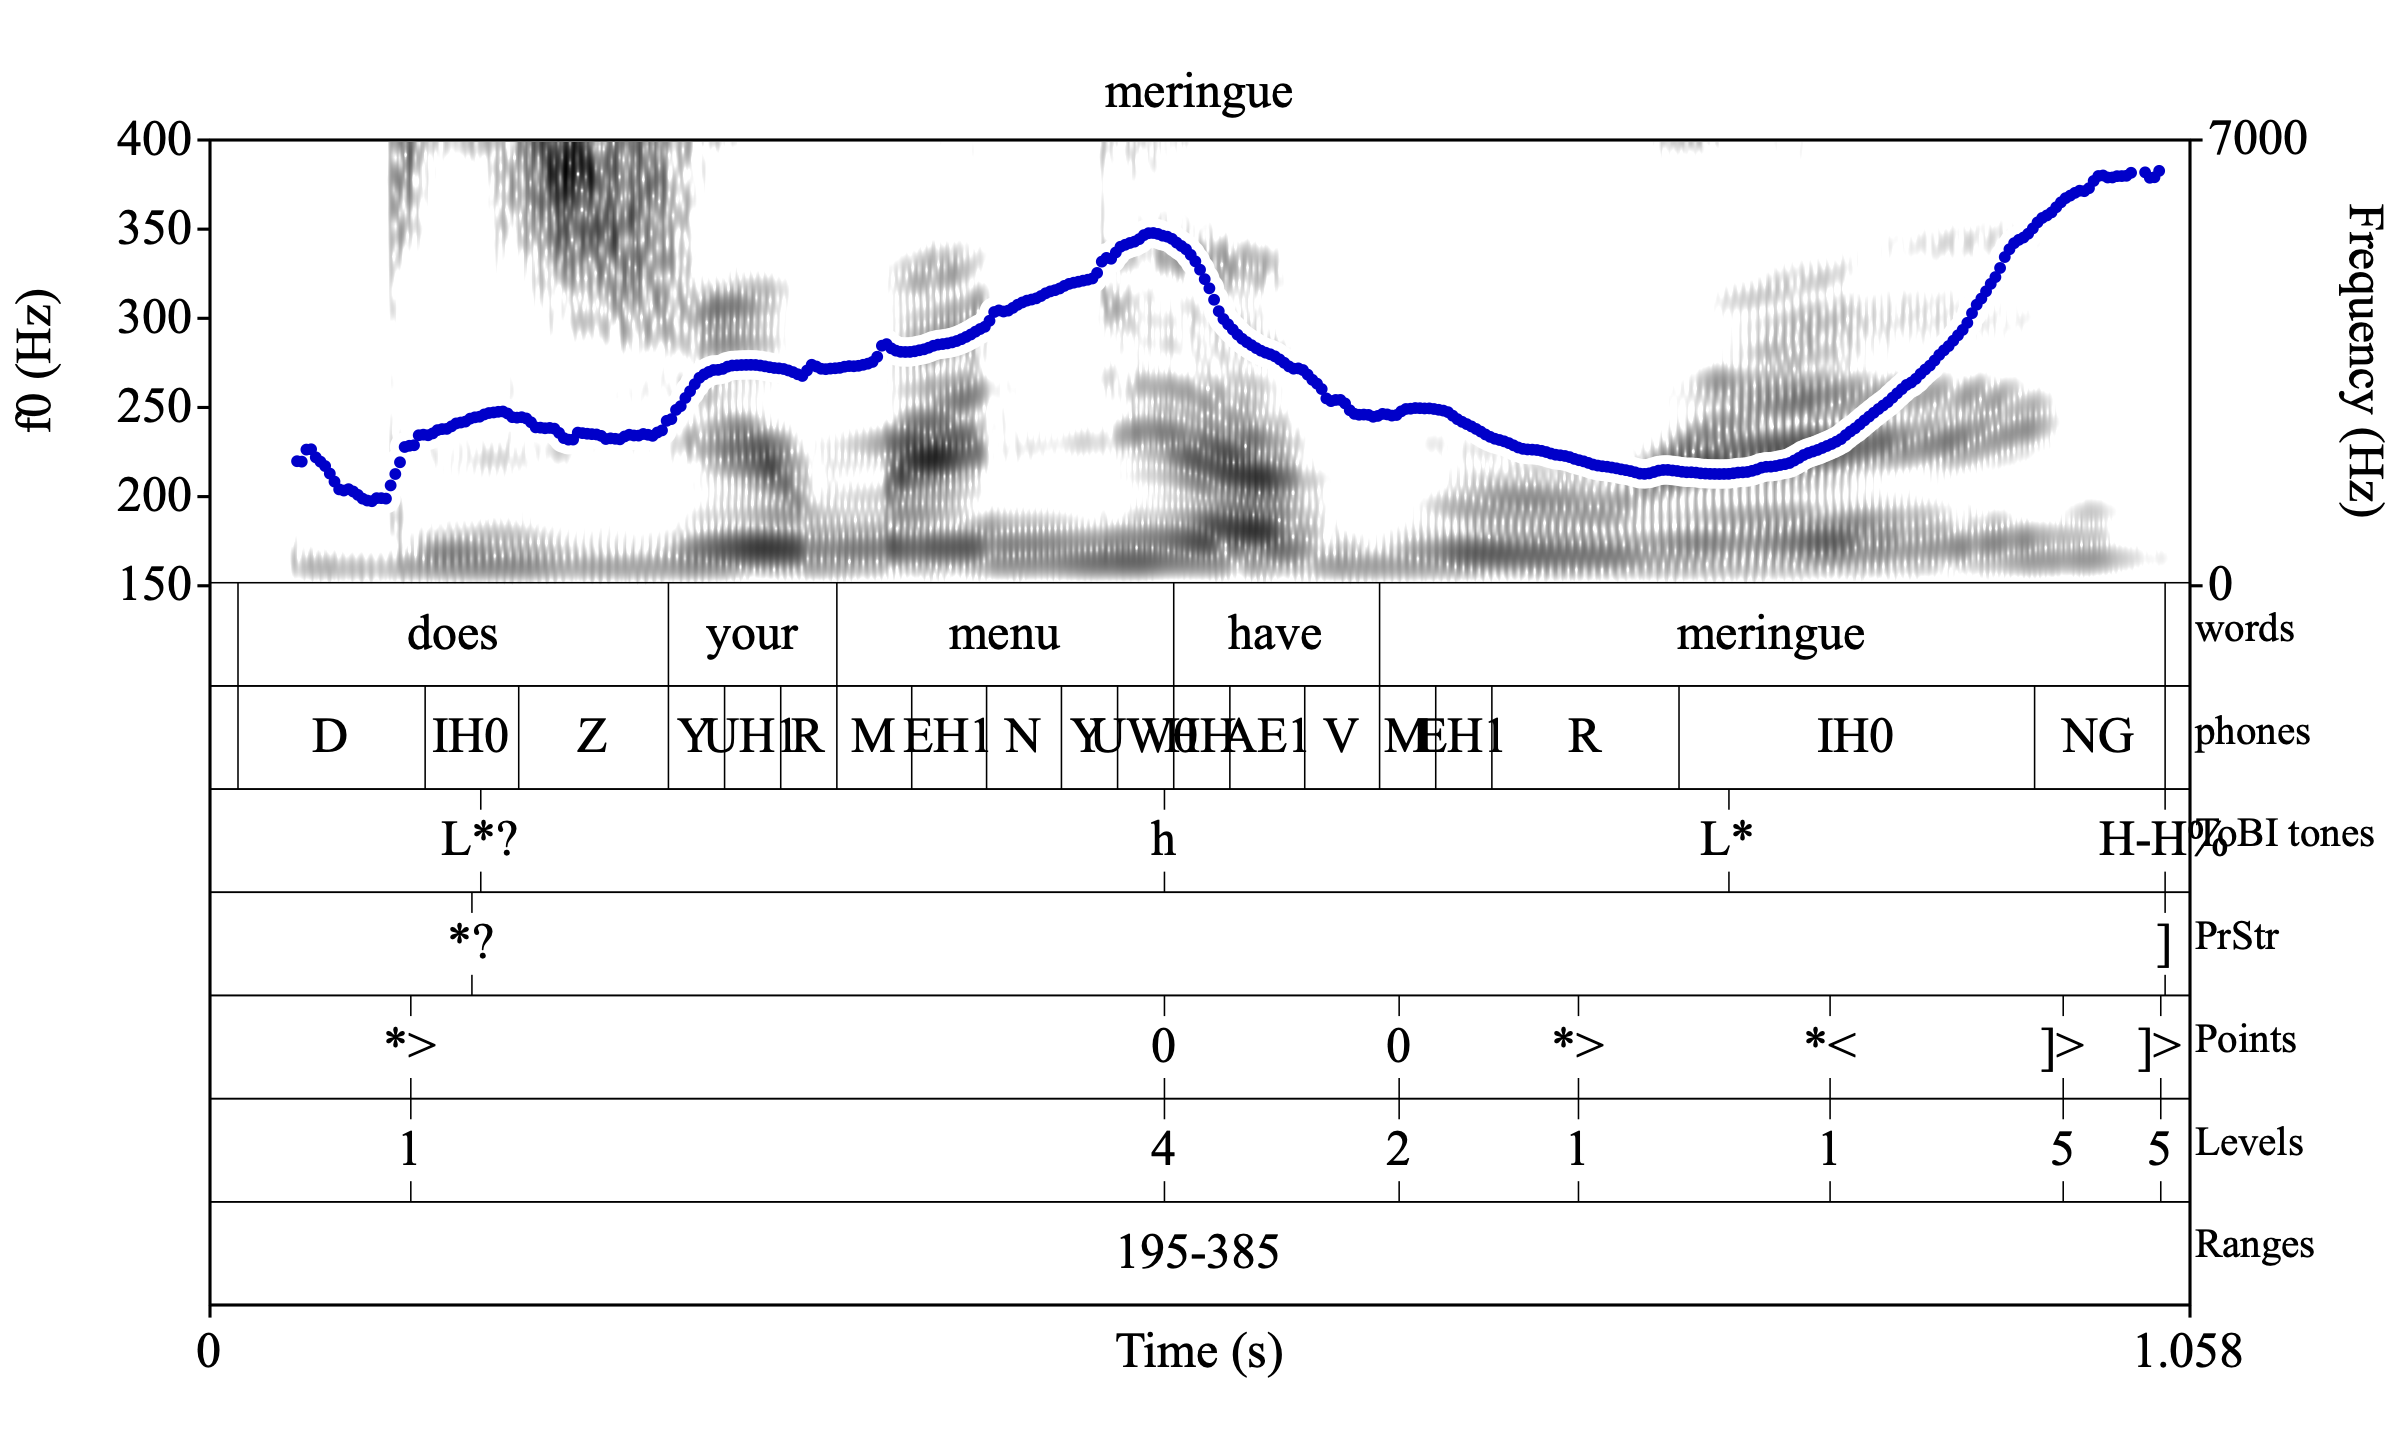
\includegraphics[width=.875\linewidth]{Usages-meringue.png}
%
\caption{A steady rise to a peak in the final (unstressed) vowel of “\langtext{menu}”, which is not perceived as prominent or at a phrase boundary.%
\label{fig:Usages meringue}%
\index{Annotated example, Usage cases!meringue}
}
\end{figure}

\begin{figure}[H]
\centering
%
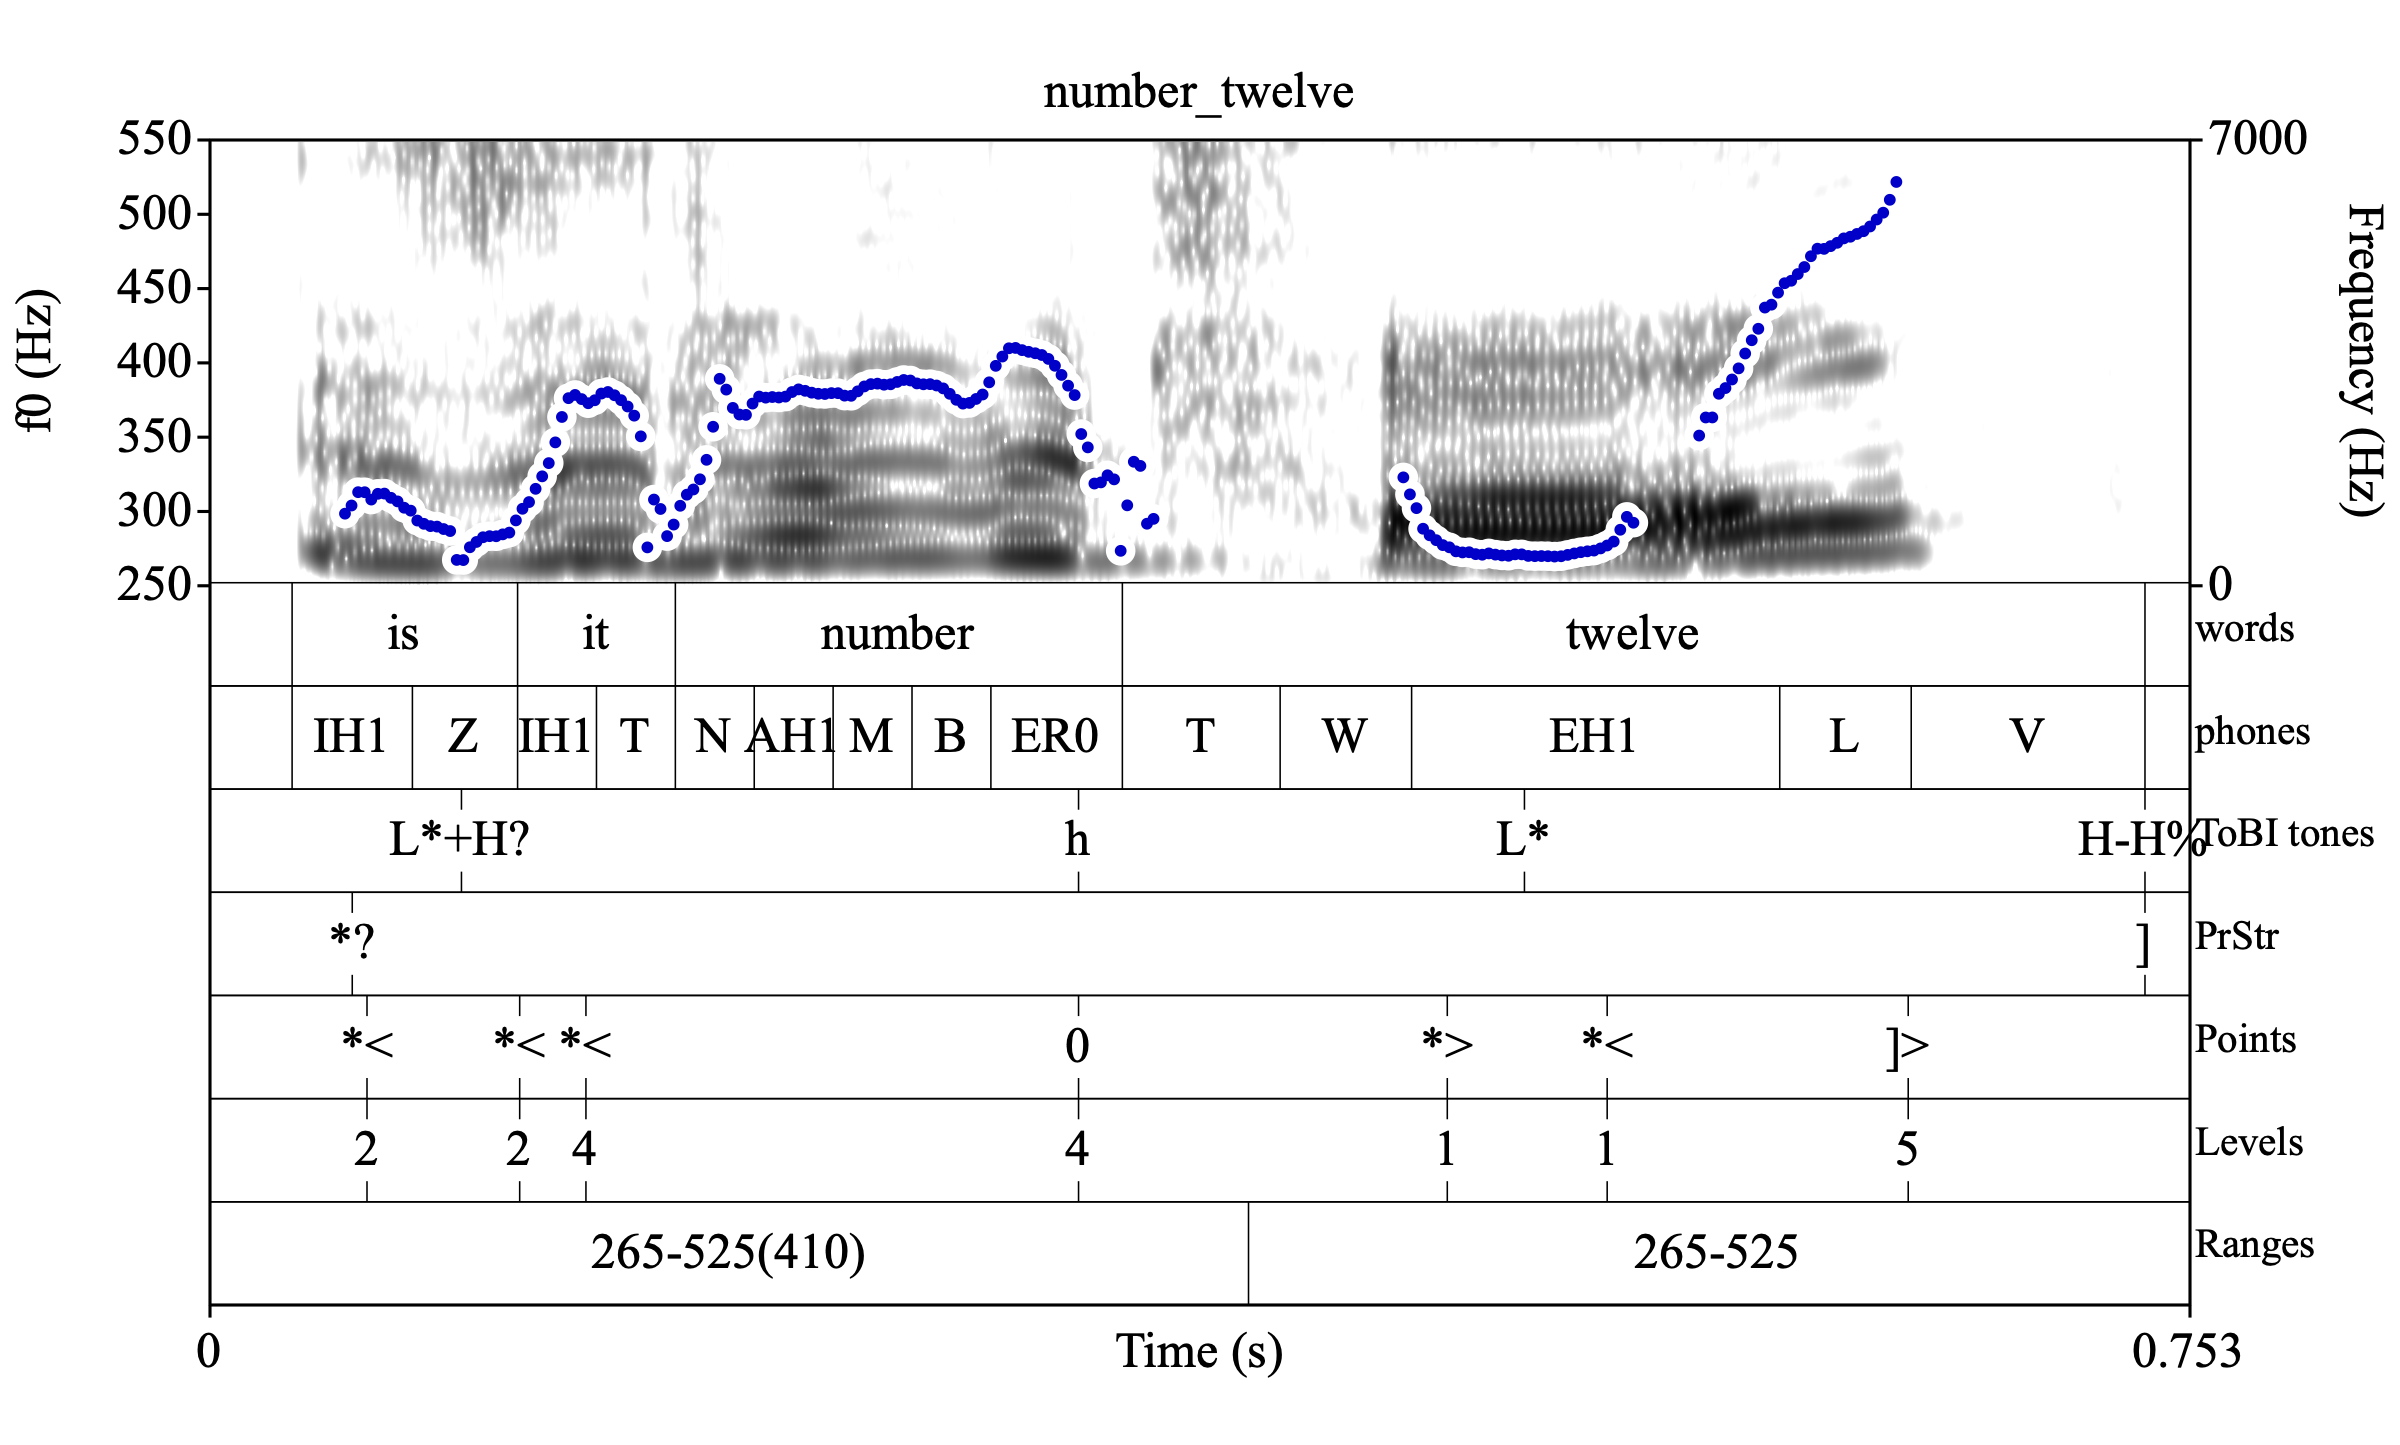
\includegraphics[width=.875\linewidth]{Usages-number_twelve.png}
%
\caption{A steady high through the final vowel of “\langtext{number}”, which is not perceived as prominent or at a phrase boundary.%
\label{fig:Usages number twelve}%
\index{Annotated example, Usage cases!number\_twelve}
}
\end{figure}


As described in \citealt{ahnzhou19}, these examples cannot be labelled using MAE\_ToBI: the rises are not tied to stressed syllables or prosodic phrase boundaries, but the MAE\_ToBI phonology requires that all pitch movements labelled on the Tones tier be associated with one of those two types of objects. As such, they are unlabellable in MAE\_ToBI, unless the labelling conventions are broken (e.g., using \textlabel{H*} in cases where there is no prominence) or set of labels is augmented (e.g., adding an \textlabel{h} label, as used in the figures above). Thus, strictly adhering to MAE\_ToBI would require not labelling these pitch movements, making it difficult to keep track of (and subsequently analyze) where these unpredicted highs occur. PoLaR labels, on the other hand, could be used for this utterance just as easily as it is used for any other utterance: all pitch movements are labelled with the Points and Levels tiers, and can be used for description and analysis.

In sum, using PoLaR to label otherwise unlabellable examples will encourage researchers to analyze patterns they might not otherwise (be able to) track. When there is no established prosodic grammar for a language\slash variety, PoLaR can be used to help build one. Additionally, using PoLaR alongside a phonological labelling system (when available) may help refine our understanding of the prosodic phonology (and may provide useful evidence for discussions about updating phonological annotation systems).


%\section{Old Stuff (partially harvested)}
%Some of these long standing difficulties arise because the phonological system of prosody is not understood deeply enough, even for well studied (varieties of) languages like Mainstream US English. There are at least three particular reasons for this state of affairs.
%\begin{enumerate}
%	\item First, some of phenomena (e.g., what counts as low\slash high within a given utterance) are currently best described in perceptual terms that rely on the intuitions of capable speakers of the target language. Speakers of a language are able to intuitively weigh\slash balance the network of the (non-deterministic) phonetic cues in the acoustic signal in perceiving intonation; however, the field has not yet been converged on a well-defined system of how this works.
%	\item Building on this, the full set of phonetic cues used by speakers of a language to identify intonational landmarks (as well as the relationships between cues) has not been fully fleshed out. This is in part because intonational labellers (again, intentionally, and by design of the system) leave such phonetic cues unmarked in the annotation, and unspoken in their discussion of their prosodic annotation system.
%	\item Finally, even within particular annotation systems, there remains a non-negligible amount of inter-labeller disagreement on which label(s) is/are appropriate for a given utterance for a variety of reasons. For example: (a) different labellers may weight different cues differently when deciding on a label, (b) the signal may underdetermine which label is appropriate, and (c) the labelling system may be insufficient to make a relevant distinction such that labellers are forced to arbitrarily choose between labels although none seem to match the speech token perfectly.
%\end{enumerate}
%What is needed first to make progress on this front is a deeper understanding of the phonetic cues and how they relate to the phonological system. By addressing this head-on, we aim to advance the field for the goals of both linguists and non-linguists alike.
%
%To this end, PoLAR is an attempt to develop a new framework that is situated both in acoustic phonetics and the language-specific basics of intonational phonology. That is, we aim to label acoustic cues (the ones labellers attend to in choosing particular labels in existing labelling systems) directly, on a number of tiers, alongside some (underspecified) phonological labels. In this way, this transcription system (PoLaR) does not require the labeller to be committed to the precise categories of any intonational phonology (e.g., MAE\_ToBI) -- as an attempt to address point (ii) above. At the same time, it still maintains a clear relationship to the broad categories proposed for in AM models (e.g., pitch accents and boundary tones), while not asking labellers to attend to a large number multiple acoustic cues (pitch height, pitch movement, etc.) into their choice of phonological label.
%
%The remainder of this document describes what human labellers in this system will do, what the computer model will do, and how the intonational phonologist can use these findings for understanding the phonetics\slash phonology interface, identifying new phonological categories….
%
%\subsection{PoLaR: A Bridge between Acoustics and Phonological Categories}
%\begin{enumerate}
%	\item Labelling these variant forms differently will help determine…
%	\begin{enumerate}
%		\item whether they occur systematically with context (speaker, meaning, surrounding prosody)
%		\item whether they matter to the listener (i.e., whether they convey information, either contrastively or gradiently)
%		\item whether they in fact contribute to the phonology.
%	\end{enumerate}
%	\item Labelling individual acoustic-phonetic cues along with pointers indicating their perceived relationship to phonological prominences and boundaries provides a bridge between the two levels, making it possible to dig down into details of the intonational system\footnote{This can be straightforwardly extended to other domains of prosody: rhythm, duration, intensity, voice quality, etc. See section [\ref{XXX}] for a brief discussion.}, and build more successful models
%	\begin{enumerate}
%		\item This will help reveal the ways in which a particular intonational contour can vary, (beyond what is predicted by purely phonological models)
%		\item Uncovering the acoustic variation will lead to a deeper understanding of which cues and cue values are employed in speech production and perceptual processing
%		\item This labelling, and the acoustic analysis it enables, provide an important stepping stone towards the development of an automatic labelling algorithm, which depends on a deeper understanding of the connection between acoustic cues and phonological categories
%	\end{enumerate}
%	\item This annotation system will provide information that will deepen our understanding of the relationship between intonational form and different levels of meaning (semantic, pragmatic, sociolinguistic, etc.)
%\end{enumerate}
%


\bibliographystyle{glossa.bst}
\bibliography{ch5.bib}

\end{document}	